\documentclass[journal]{IEEEtran}

\usepackage[normalem]{ulem}
\usepackage{mathptmx} % This is Times font

\usepackage{fancyhdr}
\usepackage{makecell}
\usepackage{array}
\usepackage{ifthen}

\usepackage{cite}
\usepackage{amsmath,amssymb,amsfonts}

\usepackage{graphicx}
\usepackage{textcomp}
\usepackage{booktabs}
\usepackage{color,soul}
\usepackage{caption}
\usepackage{commath}
\usepackage{comment}
\usepackage{paralist}
\usepackage{xcolor}
\usepackage{listings}
\usepackage[linesnumbered,ruled,vlined]{algorithm2e}
\usepackage{float}
\usepackage[hyphens]{url}
\usepackage{tabularx}
\usepackage{cleveref}

\definecolor{mGreen}{rgb}{0,0.6,0}
\definecolor{mGray}{rgb}{0.5,0.5,0.5}
\definecolor{mPurple}{rgb}{0.58,0,0.82}
\definecolor{backgroundColour}{rgb}{0.95,0.95,0.92}
\definecolor{Alizarin}{rgb}{0.93, 0.13, 0.13}

\newcolumntype{Y}{>{\raggedright\arraybackslash}X}
\newcolumntype{P}[1]{>{\raggedright\arraybackslash}p{#1}}

\lstdefinestyle{CStyle}{
    backgroundcolor=\color{backgroundColour},
    commentstyle=\color{mGreen},
    keywordstyle=\color{magenta},
    numberstyle=\tiny\color{mGray},
    stringstyle=\color{mPurple},
    basicstyle=\footnotesize,
    breakatwhitespace=false,
    breaklines=true,
    captionpos=b,
    keepspaces=true,
    numbers=left,
    numbersep=5pt,
    showspaces=false,
    showstringspaces=false,
    showtabs=false,
    tabsize=2,
    language=C
}

\newcommand{\allowcomments}{0} %set allowcomments to 1 to see comments


\ifthenelse{\equal{\allowcomments}{0}}{
\newcommand{\fm}[1]{\textcolor{blue}{}}
\newcommand{\am}[1]{\textcolor{red}{}}
\newcommand{\cc}[1]{\textcolor{green}{}}
\newcommand{\sk}[1]{\textcolor{cyan}{}}
\newcommand{\ej}[1]{\textcolor{violet}{}}
\newcommand{\hs}[1]{\textcolor{olive}{}}
\newcommand{\prit}[1]{\textcolor{orange}{}}
\newcommand{\pranati}[1]{\textcolor{brown}{}}
\newcommand{\jw}[1]{\textcolor{Alizarin}{}}
\newcommand{\sabuj}[1]{\textcolor{purple}{}}
}{
\newcommand{\fm}[1]{\textcolor{blue}{FM: #1}}
\newcommand{\am}[1]{\textcolor{red}{AM: #1}}
\newcommand{\cc}[1]{\textcolor{green}{CC: #1}}
\newcommand{\sk}[1]{\textcolor{cyan}{SK: #1}}
\newcommand{\ej}[1]{\textcolor{violet}{EJ: #1}}
\newcommand{\hs}[1]{\textcolor{olive}{HS: #1}}
\newcommand{\prit}[1]{\textcolor{orange}{PM: #1}}
\newcommand{\pranati}[1]{\textcolor{brown}{P: #1}}
\newcommand{\jw}[1]{\textcolor{Alizarin}{JW: #1}}
\newcommand{\sabuj}[1]{\textcolor{purple}{SL: #1}}
}

\hyphenation{op-tical net-works semi-conduc-tor IEEE-Xplore}
% updated with editorial comments 8/9/2021
\newcommand{\scheme}{\textsc{BoundNoC}}
\newcommand{\cpumodel}{Intel Xeon Phi 7290}
\newcommand{\opensslver}{1.1.0f}
\newcommand{\bscheme}{\textsc{B\-o\-u\-n\-d\-N\-o\-C\textsubscript{bypass}}}
\newcommand{\jscheme}{\textsc{B\-o\-u\-n\-d\-N\-o\-C\textsubscript{delay}}}
\newcommand{\rscheme}{\textsc{B\-o\-u\-n\-d\-N\-o\-C\textsubscript{rand}}}
\newcommand{\rejscheme}{\textsc{B\-o\-u\-n\-d\-N\-o\-C\textsubscript{low\_up}}}
\newcommand{\basebscheme}{\textsc{B\-a\-s\-e\-l\-i\-n\-e\-\textsubscript{bypass}}}
\newcommand{\basescheme}{\textsc{B\-a\-s\-e\-l\-i\-n\-e\-}}
\begin{document}

\title{
\scheme: A Low-Overhead Defense Against Network-On-Chip Side Channels}

\date{}

\author{\IEEEauthorblockN{Farabi Mahmud, Harpreet Singh Chawla, Chia-Che Tsai, EJ Kim, Abdullah Muzahid}\\
\IEEEauthorblockA{\textit{Department of Computer Science and Engineering, Texas A\&M University, College Station, TX, USA}} \\
\{farabi, harpreetsc, chiache, ejkim, abdullah.muzahid\}@tamu.edu}

% The paper headers
\markboth{IEEE Transactions on Computers}%
{BoundNoC}

\IEEEpubid{0000--0000/00\$00.00~\copyright~2026 IEEE}
% Remember, if you use this you must call \IEEEpubidadjcol in the second
% column for its text to clear the IEEEpubid mark.

\maketitle

\begin{abstract}
Distributed last-level cache (LLC) architectures in modern many-core processors introduce non-uniform latencies for memory access, exploitable as side-channel attacks.
These attacks use physical distance or network congestion to leak sensitive information.
We demonstrate a concrete distance-based attack on an \cpumodel{} CPU, extracting AES secret keys from OpenSSL \opensslver{}.
To counter such attacks, we propose \scheme{}, an efficient architectural defense that creates an oblivious LLC by eliminating observable differences in access time for security-sensitive memory instructions.
We present two core mechanisms: \jscheme{}, using calibrated delay, and \bscheme{}, using router bypass.
A randomized-target variant of \bscheme{}, \rscheme{}, trades determinism for lower average latency.
We implement \scheme{} in the Gem5 simulator and evaluate it on PARSEC, Rodinia, and MLPerf Tiny.
On PARSEC and Rodinia, \jscheme{} incurs 7.24\% overhead on average, while \bscheme{} shows no measurable impact over the insecure baseline.
On MLPerf Tiny, overhead for \bscheme{} ranges from $-30.5\%$ to $+9.1\%$ depending on the benchmark; \rscheme{} lowers this to $-41.5\%$ on average.

\end{abstract}

\begin{IEEEkeywords}
Computer Architecture, Multi-core System, Network-on-chip, Non Uniform Cache Access
\end{IEEEkeywords}


\section{Introduction}
\label{sec:intro}
Large-scale multicore architectures have become the backbone of high performance computing systems.
To meet the demand of so many cores, large-scale multicores are equipped with a large last level cache (LLC).
For example, AMD EPYC Genoa-X 9648X comes with 1.2GB 3D V-Cache as LLC, whereas Intel's Granite Rapids comes with more than 512 MB of LLC~\cite{intel-hotchips-23} in a 144-core processor.
Such LLCs are typically distributed over multiple banks connected through a network-on-chip (NoC) to reduce access latency, ease manufacturing complexities, and improve core isolation.
Distributed LLC improves memory level parallelism by allowing multiple concurrent requests to different banks.
However, accesses to different banks incur different latencies, which is why this type of architecture is referred to as a Non-Uniform Cache Access (NUCA) architecture.

A side channel is a security vulnerability where an attacker infers secrets through observable physical characteristics of a system, such as timing.
NUCA architectures have been subject to numerous security vulnerabilities that exploit the non-uniformity of access latencies.
For example, Don't Mesh Around~\cite{dont-mess-around} and MeshUp~\cite{meshup} showed a contention-based cache side channel attack in the mesh interconnect of a NUCA architecture.
Following the trend of earlier works, Attack of Knights (AoK) introduced a distance-based cache side channel attack in a similar architecture~\cite{mahmud2022distancebased}.
These attacks pose a significant threat to security-sensitive applications running on NUCA architectures.
Therefore, it is imperative to defend against these vulnerabilities caused by the side channel in caches of NUCA architecture.

\IEEEpubidadjcol

While several defense mechanisms have been proposed, there are a few existing techniques to defend against NoC-based cache side channel attacks.
For example, SurfNoc~\cite{wassel2013surfnoc} proposed to separate packets based on their application domains and forward packets from the same domain at the same time.
Gossip Noc~\cite{reinbrecht2016gossip} proposed to filter out attack packets and change their routing functions.
Kar et al.~\cite{remapping-llc} proposed to remap LLC banks dynamically to defend against contention-based cache side channel attacks.
However, these solutions have performance, area, and power overhead.
Moreover, these techniques do not defend against distance-based side channel attacks in NUCA architectures (like AoK~\cite{mahmud2022distancebased}).
A related line of research, Oblivious RAM (ORAM)~\cite{oram,phantom,sanctum}, addresses these attacks by hiding memory access patterns entirely.
However, hardware ORAM implementations incur prohibitive overhead.
For example, one such configuration, Phantom~\cite{phantom} has $6\times$ performance overhead compared to the baseline system.
Therefore, our goal is to devise a low-overhead defense mechanism against any side channel in a NUCA architecture's cache.

We believe that a side channel (whether based on congestion, contention or distance) in the NUCA architecture can be prevented if we could turn the LLC into essentially an oblivious cache, i.e., make the latency of all relevant cache accesses constant so that the attacker cannot infer any access pattern from the latency differences.
Based on this intuition, in this paper, we propose two defense techniques---\jscheme\ and \bscheme---which make the latency of cache accesses constant regardless of congestion, contention or distance difference.
Collectively, we refer to the proposed techniques as \scheme.

\jscheme\ aims to make the latency of accessing {\em any} LLC bank to be as long as the longest LLC latency, so that the LLC does not exhibit any timing difference.
To make any LLC bank latency equal to the longest LLC latency (say, $T_{worst}$), \jscheme\ adds some delay to the original access latency (say, $T_{orig}$).
An appropriate amount of delay (i.e., $T_{worst}-T_{orig}$) is added right before the LLC bank sends the requested data back to the core.
\jscheme\ is simple and intuitive but hurts performance as it slows down LLC accesses significantly.

To reduce the performance overhead, we must not make the constant latency of LLC accesses equal to $T_{worst}$.
Therefore, we propose \bscheme.
Here, we make the following observation---{\em instead of making every LLC access have the latency $T_{worst}$, we can reduce the worst case latency to a much lower latency and then make every LLC access latency equal to that}.
There have been studies on reducing packet latency in NoC designs.
One class of techniques, called Router Bypass~\cite{krishna2013breaking,chen2013smart,krishna2013single,kwon2017opensmart,yang2017task,perez2019smart++,zong2016doart,ma2021latency}, opens up an opportunity for speeding up accesses to the farthest banks, thereby reducing the worst case latency.
For instance, by applying the router bypass technique to the farthest bank, we can reduce $T_{worst}$ latency to a much lower latency $T_{low}$.
\bscheme\ eliminates LLC access latency differences by making every latency equal to $T_{low}$.
\bscheme\ works by adding delay to accesses to nearby LLC banks (since the access latency of nearby banks is presumably lower than $T_{low}$) and a combination of router bypass and delay (if needed) to accesses to the distant LLC banks.
Delay and router bypass mechanisms are applied by modifying the NoC router hardware.
Although router bypass has been proposed before, to the best of our knowledge, this is the {\em first} work that uses it as a security solution.

We implement our proposed techniques using Gem5~\cite{binkert2011gem5} and Garnet~\cite{agarwal2009garnet} simulators.
We show the impact of both \jscheme\ and \bscheme\ using different workloads from the PARSEC~\cite{bienia2008parsec} and Rodinia~\cite{che2009rodinia} benchmark suites.
Finally, we also show how both schemes defend against a NUCA cache side channel attack (whether it is congestion, contention or distance-based) by eliminating latency differences of LLC accesses.

We make the following contributions:
\begin{compactitem}
    \item We analyze existing NUCA cache side channel attacks---including
    congestion, contention, and distance-based variants---and
    establish the necessary and sufficient conditions for an effective defense.

    \item We propose two defense techniques against NUCA cache side channel attacks---\jscheme\ and \bscheme.
    Both techniques ensure constant-time LLC accesses (with a combination of router bypass and delay), essentially converting the LLC into an oblivious one.
    {\em This is the first use of router bypass mechanism for cache security}.

    \item We implement our proposed defenses in the Gem5~\cite{binkert2011gem5} architectural simulator and evaluate them using benchmarks from the PARSEC~\cite{bienia2008parsec} and Rodinia~\cite{che2009rodinia} benchmark suites.
    Our results indicate that, on average, with minimal NoC hardware modification,
    \jscheme\ adds $17.04\%$ runtime overhead compared to a baseline vulnerable system while \bscheme\ does not cause any runtime degradation at all.
\end{compactitem}

The remainder of this paper is organized as follows.
Section~\ref{sec:back} provides background and related work.
Section~\ref{sec:threatmodel} describes our threat model.
Section~\ref{sec:attack-overview} presents an overview of NUCA side channel attacks.
Section~\ref{sec:desc} describes \scheme{} in detail.
Section~\ref{sec:impl} presents implementation details.
Section~\ref{sec:security} provides a security analysis.
Section~\ref{sec:eval} presents our evaluation results.
Section~\ref{sec:conclusion} concludes the paper.



\section{Background and Related Work}
\label{sec:back}
NUCA architectures introduce performance and security trade-offs that motivate the design of \scheme{}.
This section provides the necessary background on these trade-offs and surveys related work.

\subsection{NUCA Architecture}
Modern multicore processors employ increasingly large cache hierarchies to bridge the performance gap between CPU cores and main memory~\cite{muralimanohar2007interconnect, jaleel2006last}.
As core counts and bandwidth demands increase, last-level caches (LLCs) are often physically distributed into multiple banks or slices rather than implemented as a single monolithic structure.
These LLC banks are connected through an on-chip interconnect or network-on-chip (NoC), which allows multiple cores to access different cache banks concurrently.
This physical distribution gives rise to Non-Uniform Cache Access (NUCA) architectures, where the latency of an LLC access depends on the physical and network distance between the requesting core and the target LLC bank~\cite{kim2002adaptive}.
For example, an access to a nearby LLC bank may traverse only a few NoC hops, while an access to a distant bank may traverse many more.
Consequently, even when two accesses both hit in the LLC, they may exhibit different access latencies due solely to their locations in the on-chip network.

On-chip interconnects can be organized using several topologies, including crossbars, rings, meshes, tori, and 3D tori~\cite{jerger2009chip}.
A typical NoC consists of nodes connected by physical links.
Each node may contain one or more CPU cores, private caches, shared LLC banks, a router, a network interface, coherence-directory state, or memory-controller logic.
A typical NoC router consists of input buffers, a crossbar switch, routing logic, and flow-control logic.
Packets traverse the network hop-by-hop, spending at least one cycle per router for arbitration and switching.
Communication between nodes occurs through packets routed according to the network routing protocol and regulated by flow-control mechanisms.

Among commercial processors, Intel Nehalem used a ring-based interconnect for Xeon processors with up to eight cores, while later Intel Skylake-SP and Skylake-X processors adopted mesh interconnects~\cite{kommrusch2021optimizing,dont-mess-around}.
In distributed LLC designs, an address is typically mapped to an LLC slice and associated coherence metadata.
In Intel manycore systems, this metadata is maintained by Caching and Homing Agents (CHAs), which track the location, ownership, and coherence state of cache lines.
Since CHAs and LLC banks are physically distributed across the chip, accesses to different CHAs or LLC banks can incur different NoC traversal latencies.
This non-uniformity is beneficial for scalability and performance, but it also creates a timing signal that can be exploited by NUCA side-channel attacks.

\subsection{Cache Side-Channel Attacks}
\label{sec:back_sidechannel}
Hardware side-channel attacks exploit observable microarchitectural effects to infer secret-dependent behavior.
Examples of such observable effects include cache hits and misses, access latency in TLBs, caches, and DRAM, and contention in shared hardware structures.
In a typical side-channel attack, the victim performs secret-dependent operations that modify the state or timing behavior of a shared resource, and the attacker observes these changes to infer information about the secret of the victim.

Cache side-channel attacks are among the most widely studied hardware side channels.
They are commonly categorized based on how the attacker prepares the cache state and how the attacker measures the victim-induced change.

\textbf{Prime+Probe~\cite{liu2015last,schwarz2017malware, brasser2017software,kayaalp2016high,aciiccmez2008vulnerability,tromer2010efficient,osvik2006cache,neve2006advances}:}
In Prime+Probe, the attacker first fills selected cache sets with its own cache lines during the prime phase.
After the victim executes, the attacker probes the same sets and measures whether its cache lines were evicted.
Evictions reveal that the victim accessed data mapping to the same cache sets, allowing the attacker to infer secret-dependent memory behavior.

\textbf{Flush+Reload~\cite{gullasch2011cache,gruss2015cache,zhang2014cross,yarom2014recovering,van2015just,irazoqui2014wait,yarom2014flush+}:}
Flush+Reload uses the \texttt{CLFLUSH} instruction to evict a shared cache line and later reloads the same line to determine whether the victim accessed it.
A fast reload indicates that the victim brought the line back into the cache.
This attack provides high spatial and temporal resolution, but it requires the attacker and victim to share memory at cache-line granularity.

\textbf{Flush+Flush~\cite{gruss2016flush+}:}
Flush+Flush exploits the execution-time difference of the \texttt{CLFLUSH} instruction itself.
Because flushing a cached line can take a different amount of time than flushing an uncached line, the attacker can infer whether the victim accessed the target line without explicitly reloading it.
This makes Flush+Flush stealthier than attacks that rely on measuring reload latency.

Recent microarchitectural attacks further show that timing leakage extends beyond traditional cache-set contention; these works are complementary to \scheme{} and target different leakage sources.
For example, HertzBleed~\cite{hertzbleed} shows that dynamic voltage and frequency scaling can turn data-dependent power behavior into timing leakage.
GoFetch~\cite{gofetch} shows that hardware prefetching can undermine constant-time cryptographic implementations.
SQUIP~\cite{squip} exploits contention in shared microarchitectural queues.
Recent defenses such as ClepsydraCache~\cite{clepsydra}, randomized caches, and Goldilocks~\cite{goldilocks} address specific leakage sources such as cache eviction behavior, randomized cache mapping, or frequency-induced timing variation.

\subsection{Existing Defenses and Their Limitations} \label{sec:back_defenses}
Several classes of defenses have been proposed against cache side-channel attacks.
Timing obfuscation techniques perturb or reduce the precision of timing measurements, making it harder for the attacker to decode secret-dependent behavior~\cite{zhang2011predictive,godfrey2013server}.
Partitioning and isolation mechanisms prevent attackers and victims from sharing the same cache
resources~\cite{kiriansky2018dawg,liu2016catalyst,wang2007new,kim2012stealthmem}.
Oblivious RAM (ORAM)~\cite{oram,phantom,sanctum} can mitigate a broad range of access-pattern side channels by hiding memory access patterns, but it generally incurs significant performance and storage overhead due to memory reshuffling and metadata management.
For example, Phantom~\cite{phantom} has $6\times$ performance overhead compared to the baseline system.

Prior defenses against NoC-based side-channel attacks generally attempt to segregate, schedule, or distribute network traffic.
SurfNoc~\cite{wassel2013surfnoc} separates packets based on their application domains and forwards packets from the same domain at the same time.
Reinbrecht et al.~\cite{reinbrecht2016gossip} proposed GossipNoC, which dynamically changes the routing algorithm when abnormal network behavior is detected.
Kar et al.~\cite{remapping-llc} proposed dynamic remapping of LLC banks to defend against contention-based cache side-channel attacks.
Such defenses can reduce interference-based channels because those attacks depend on shared NoC resources or traffic contention.
However, they do not eliminate the fundamental non-uniformity of LLC access latency in NUCA architectures.
In particular, even if contention is removed, a victim access to a nearby LLC bank or CHA can still complete faster than an access to a distant bank or CHA.
This distance-dependent timing signal motivates the need for a defense that equalizes LLC-hit latency rather than only reducing network interference.

\subsection{NoC-Based Side-Channel Attacks}
NoC-based side channels exploit timing or throughput variations in the on-chip interconnect.
In Multi-Processor System-on-Chips (MPSoCs), Reinbrecht \textit{et al.} showed that NoC behavior can be leveraged for Prime+Probe-style cache side-channel attacks~\cite{reinbrecht2016side}.
In this attack, the attacker monitors throughput changes to detect when a cryptographic victim accesses cache lines for key-dependent lookups, and then uses this information to initiate the probe phase.

More recent attacks have demonstrated that timing channels also exist in commercial CPU interconnects.
Paccagnella \textit{et al.} developed timing side-channel attacks on CPU ring interconnects by exploiting NoC and cache contention~\cite{paccagnella2021lotr}.
Dai \textit{et al.} showed that contention in a 2D mesh interconnect of a NUCA system can create measurable timing differences, enabling both covert and side-channel attacks~\cite{dont-mess-around}.
In their attack, the transmitter creates traffic contention on shared NoC paths to encode information, while the attacker detects the transmitted value by measuring access latency.
Similarly, MeshUp exploits mesh-interconnect behavior to construct a stateless cache side channel on modern CPU meshes~\cite{meshup}.

Distance-based NUCA attacks do not rely solely on cache-set conflicts, replacement policies, or eviction behavior.
Instead, they exploit observable latency differences among LLC-hit accesses to different LLC banks or CHAs, where the latency variation arises from NoC distance, congestion, or both.
\scheme{} specifically targets this class of leakage by equalizing the latency of security-sensitive LLC-hit accesses in distributed LLC architectures using delay and/or router-bypass mechanisms.

\subsection{Comparison of Cache Side-Channel Attack Models}
\begin{figure}[t]
    \centering
    \includegraphics[width=\columnwidth]{figs/attack-comparison.pdf}
    \caption{Comparison of communication models between the transmitter (victim) and receiver (attacker) in three cache side-channel attacks: (a) Prime+Probe~\cite{percival2005cache}, (b) Dai et al.~\cite{dont-mess-around}, and (c) the distance-based NUCA attack of     AoK~\cite{mahmud2022distancebased}.}
    \label{fig:attack-comparison}
\end{figure}

\begin{table}[t]
    \centering
    \scriptsize
    \setlength{\tabcolsep}{2.5pt}
    \renewcommand{\arraystretch}{1.18}
    \begin{tabularx}{\columnwidth}{|P{0.58in}|Y|Y|Y|}
        \hline
        \textbf{Property}
        & \makecell[c]{\textbf{Prime+Probe}~\cite{percival2005cache}}
        & \makecell[c]{\textbf{Dai et al.}~\cite{dont-mess-around}}
        & \makecell[c]{\textbf{AoK}~\cite{mahmud2022distancebased}} \\
        \hline \hline
        Target arch.
        & Any cache or NUCA
        & Ring-based mesh
        & Multi-hop mesh \\
        \hline
        Covert?
        & No
        & Yes
        & No \\
        \hline
        Attack model
        & Eviction-based contention
        & Traffic-based contention
        & Distance-based timing \\
        \hline
        Exploit target
        & Shared cache sets
        & Shared NoC paths/rings
        & LLC bank/CHA distance \\
        \hline
        Defenses
        & ORAM; partitioning
        & ORAM; clustering; scheduling
        & ORAM; delay/bypass \\
        \hline
    \end{tabularx}
    \caption{Comparison of representative cache and NoC side-channel attacks and their applicable defense categories.}
    \label{tab:attack_differences}
\end{table}

We now compare the communication models of three representative cache side-channel attacks: Prime+Probe~\cite{percival2005cache}, the NoC-contention attack by Dai \textit{et al.}~\cite{dont-mess-around}, and the distance-based NUCA attack demonstrated by Attack of Knights (AoK)~\cite{mahmud2022distancebased}.
Figure~\ref{fig:attack-comparison} illustrates the communication relationship between the transmitter (victim) and the receiver (attacker) in these attacks, while Table~\ref{tab:attack_differences} summarizes their key differences.

Prime+Probe is an eviction-based contention channel.
The victim transmits information implicitly by evicting cache lines of the attacker from shared cache sets, and the attacker decodes the information by measuring which of its lines were evicted.
In contrast, the attack by Dai \textit{et al.} is a traffic-based contention channel.
The transmitter generates NoC traffic on paths shared with the receiver, and the receiver detects the transmitted value by measuring the latency increase caused by network contention.

AoK follows a different communication model.
Rather than relying on eviction-based cache contention or deliberate NoC traffic contention, AoK exploits distance-dependent timing differences in NUCA architectures.
The attacker observes the timing of victim operations and infers whether the victim accessed a near or far LLC bank or CHA.
Therefore, a distance-based NUCA attack requires an architecture in which LLC-hit accesses to different banks or CHAs produce distinguishable timing differences, such as a multi-hop mesh-based manycore processor.

This distinction has important implications for defenses.
Because Prime+Probe and the attack by Dai \textit{et al.} rely on shared resources, they can be mitigated by partitioning, clustering, scheduling, or otherwise reducing resource sharing between the attacker and victim.
However, distance-based NUCA attacks cannot be fully eliminated by partitioning or clustering alone, as long as the attacker can time victim operations.
Their success depends on the observability of latency differences, not necessarily on direct contention over a shared cache set or NoC path.
ORAM~\cite{oram} can mitigate all three classes of attacks by hiding memory access patterns, but it generally incurs high overhead.
\scheme{} therefore takes a more targeted approach: it removes the timing signal exploited by NUCA attacks by enforcing constant latency for security-sensitive LLC-hit accesses, without requiring memory access pattern shuffling or the associated storage overhead.



\section{Threat Model and Assumptions}
\label{sec:threatmodel}
In this paper, we assume that the attacker targets a NUCA architecture with a multi-hop mesh interconnect.

\textbf{Attacker Goal:}
The attacker aims to infer secret-dependent memory access patterns of a victim program by observing LLC access latency differences in a NUCA architecture.

\textbf{Attacker Capabilities:}
The attacker can identify a vulnerable access pattern either through binary profiling or directly from the source code if available.
The attacker can time sensitive operations in the victim program through interaction with the victim.
Examples include sending or receiving messages through the network or IPC, detecting modifications of shared variables, or using other side channels.
The attacker may or may not have access to an accurate timing source (e.g., \texttt{rdtsc}); if not, alternatives such as counting threads can be used instead.
We also assume that the attacker does not have root privileges.

\textbf{Attacker Knowledge:}
The attacker knows the general microarchitectural properties of the target system, including the NoC topology and LLC bank mapping, but need not know the source code of the victim.

\textbf{Trust Assumptions:}
The proposed defense techniques assume a trusted CPU and OS.
Defending against a malicious CPU or OS is outside the scope of this work, as it would require a fundamentally different threat model (e.g., trusted execution environments).

\textbf{Scope and Limitations:}
This work does not defend against side channels in which the non-uniformity of the cache architecture is not the source of the timing difference.
The following are considered out of scope:
\begin{compactitem}
    \item Timing channels based on cache hit/miss differences~\cite{osvik2006cache};
    \item Inference channels based on cache eviction~\cite{yarom2014flush+,irazoqui2015s,liu2015last,gruss2015cache} and replacement policies~\cite{lru-sidechannel};
    \item Timing channels based on data-independent execution time differences in single-core architectures.
\end{compactitem}
For these side channels, we assume the victim program is already protected using existing solutions, such as cache partitioning~\cite{kiriansky2018dawg} or oblivious execution~\cite{oram,phantom}.

Finally, a transient execution attack~\cite{spectre,meltdown} could potentially exploit this side channel to leak secrets obtained during transient execution.
However, such an attack faces a fundamental challenge: the transient execution window is short and CPU microarchitectural noise makes timing unreliable.
We therefore consider transient execution attacks out of scope and leave their interaction with NUCA timing channels as future work.



% \section{A Distance-Based NUCA Side Channel}
% \label{sec:attack}
% \input{attack}

\section{Attack Overview}
\label{sec:attack-overview}
\input{attack_overview}

\section{\scheme{}: A Timing-Based Defense} % with \scheme}
\label{sec:desc}
In this section, we describe the design of \scheme{} as a timing-based defense against NUCA side-channel attacks.

\subsection{Network-on-Chip and Router Bypass} \label{sec-noc-background}
Network-on-chip (NoC) has become a scalable communication fabric for large-scale NUCA architectures.
In a NoC, Network Interfaces (NIs) connect each core/cache tile to the network through a set of routers.
A packet travels from the NI of the source tile through the network routers to the NI of the destination tile.
A router consists of several pipeline stages, including routing computation, virtual channel allocation, switch arbitration, and switch traversal, followed by link traversal.
Consequently, packets traverse the network hop-by-hop through a multi-stage router pipeline.

To reduce packet latency, router bypassing has been proposed in various forms~\cite{krishna2013breaking}.
Express Virtual Channels (EVCs) virtually bridge two nodes across multiple bypass routers so that a packet traverses a bypass router in one cycle, without virtual channel or switch arbitration.
Building on EVC, SMART~\cite{krishna2013breaking} enables a single-cycle multi-hop data path from source to destination.
In this work, we leverage the bypass mechanism to selectively regulate packet latency for mitigating NUCA attacks (Section~\ref{sec-bscheme}).
This is the \emph{first} use of a bypass mechanism to resolve a distance-based NUCA cache side-channel attack.

\subsection{Scope of \scheme} \label{sec-scope}
We now explain which memory accesses \scheme{} targets and why.

\scheme{} is applied only to accesses that cause LLC hits.
Accesses that hit in L1D never reach the LLC and are therefore unaffected by LLC bank distances.
Accesses that miss in the LLC incur DRAM latency, which dominates any NoC traversal difference and cannot be exploited for a distance-based or congestion-based NUCA attack.
We refer to any load instruction that causes an LLC hit as a \emph{Security Sensitive} instruction, also called a Secure LD.

\scheme{} does not target store instructions for two reasons.
First, from the perspective of an attacker, a store instruction is harder to time due to write buffers and the inability to use fence instructions freely.
Second, an attacker cannot enforce LLC hits for store instructions: when the attacker brings a cache line to the LLC and the victim later stores to it, the store generates coherence invalidations rather than an LLC hit, making a NUCA attack infeasible.

\subsubsection{Defending Against Congestion-Based Attacks}
Congestion-based attacks rely on observable latency increases caused by deliberate NoC congestion on the communication path of the victim~\cite{meshup,dont-mess-around}.
To defend against these attacks, \scheme{} ensures that all packets are delivered within a fixed latency bound regardless of congestion.
Setting this bound to $T_{worst}$ provides security but hurts performance (Section~\ref{sec:perf-overhead}).
Instead, \scheme{} uses a lower bound $T_{low}$ maintained even in the presence of congestion, as described in Section~\ref{sec-bscheme}.

\subsubsection{Defending Against Distance-Based Attacks}
Distance-based attacks~\cite{mahmud2022distancebased} exploit latency differences between LLC accesses to near and far banks.
Unlike congestion-based attacks, they cannot be resolved by cache partitioning or isolation alone.
\scheme{} eliminates the timing signal by ensuring that all Security Sensitive LLC-hit accesses complete in constant time, regardless of the distance to the target LLC bank or CHA.

\subsection{Overview of \scheme} \label{sec-overview}

\begin{figure}[t]
    \centering
    \includegraphics[width=\columnwidth]{figs/Camouflage-Overview.pdf}
    \caption{Overview of \scheme{}.
    \scheme{} hardware ensures fixed latency for LLC memory accesses using delay and/or bypass techniques.}
    \label{fig:overview}
\end{figure}

Figure~\ref{fig:overview} shows an overview of \scheme{}.
When a core executes a Security Sensitive instruction, it sends a request to the CHA through the NI.
The CHA determines the destination tile and sends a forwarding request.
\scheme{} hardware at the destination NI checks the expected round-trip latency against the target latency.

\scheme{} chooses the target latency based on either the worst-case round-trip latency to the furthest LLC bank (\jscheme{}) or the minimum achievable round-trip latency to the furthest LLC bank using bypass (\bscheme{}).

With \jscheme{}, the destination NI uses normal routing to send back the response, and the source NI adds the necessary delay upon receiving it.
With \bscheme{}, if the expected round-trip latency exceeds $T_{low}$, the destination NI sends the response through a bypass channel to expedite delivery.
Upon receiving the response, the source NI adds any remaining delay needed to meet $T_{low}$.
In both schemes, \scheme{} hardware ensures constant LLC-hit latency for Security Sensitive instructions, preventing any NUCA timing attack.

\subsection{\jscheme} \label{sec-jscheme}
\jscheme{} is the simplest approach to ensuring constant LLC access latency.
It sets the target latency to the worst-case round-trip latency $T_{worst}$ from the source NI to any destination NI, and delays every response until that time elapses.

For a 2D mesh topology, the worst-case scenario occurs when the source NI is at one corner and the destination NI is at the opposite corner.
Since the worst-case latency varies with network traffic, $T_{worst}$ is determined under a heavily congested but not yet saturated network.

Using Booksim 2.0~\cite{booksim}, we simulate an $8\times8$ mesh and measure round-trip latency at varying injection rates (Figure~\ref{fig:jitter-threshold}).
We set $T_{worst}=100$ cycles, corresponding to the round-trip latency just before network saturation (injection rate 0.357), at which the one-way network latency is under 50 cycles on average.
We do not select a point at or above saturation because at saturation the round-trip latency becomes non-deterministic and prohibitively large, making a distance-based NUCA attack impossible regardless.

\begin{figure}[t]
    \centering
    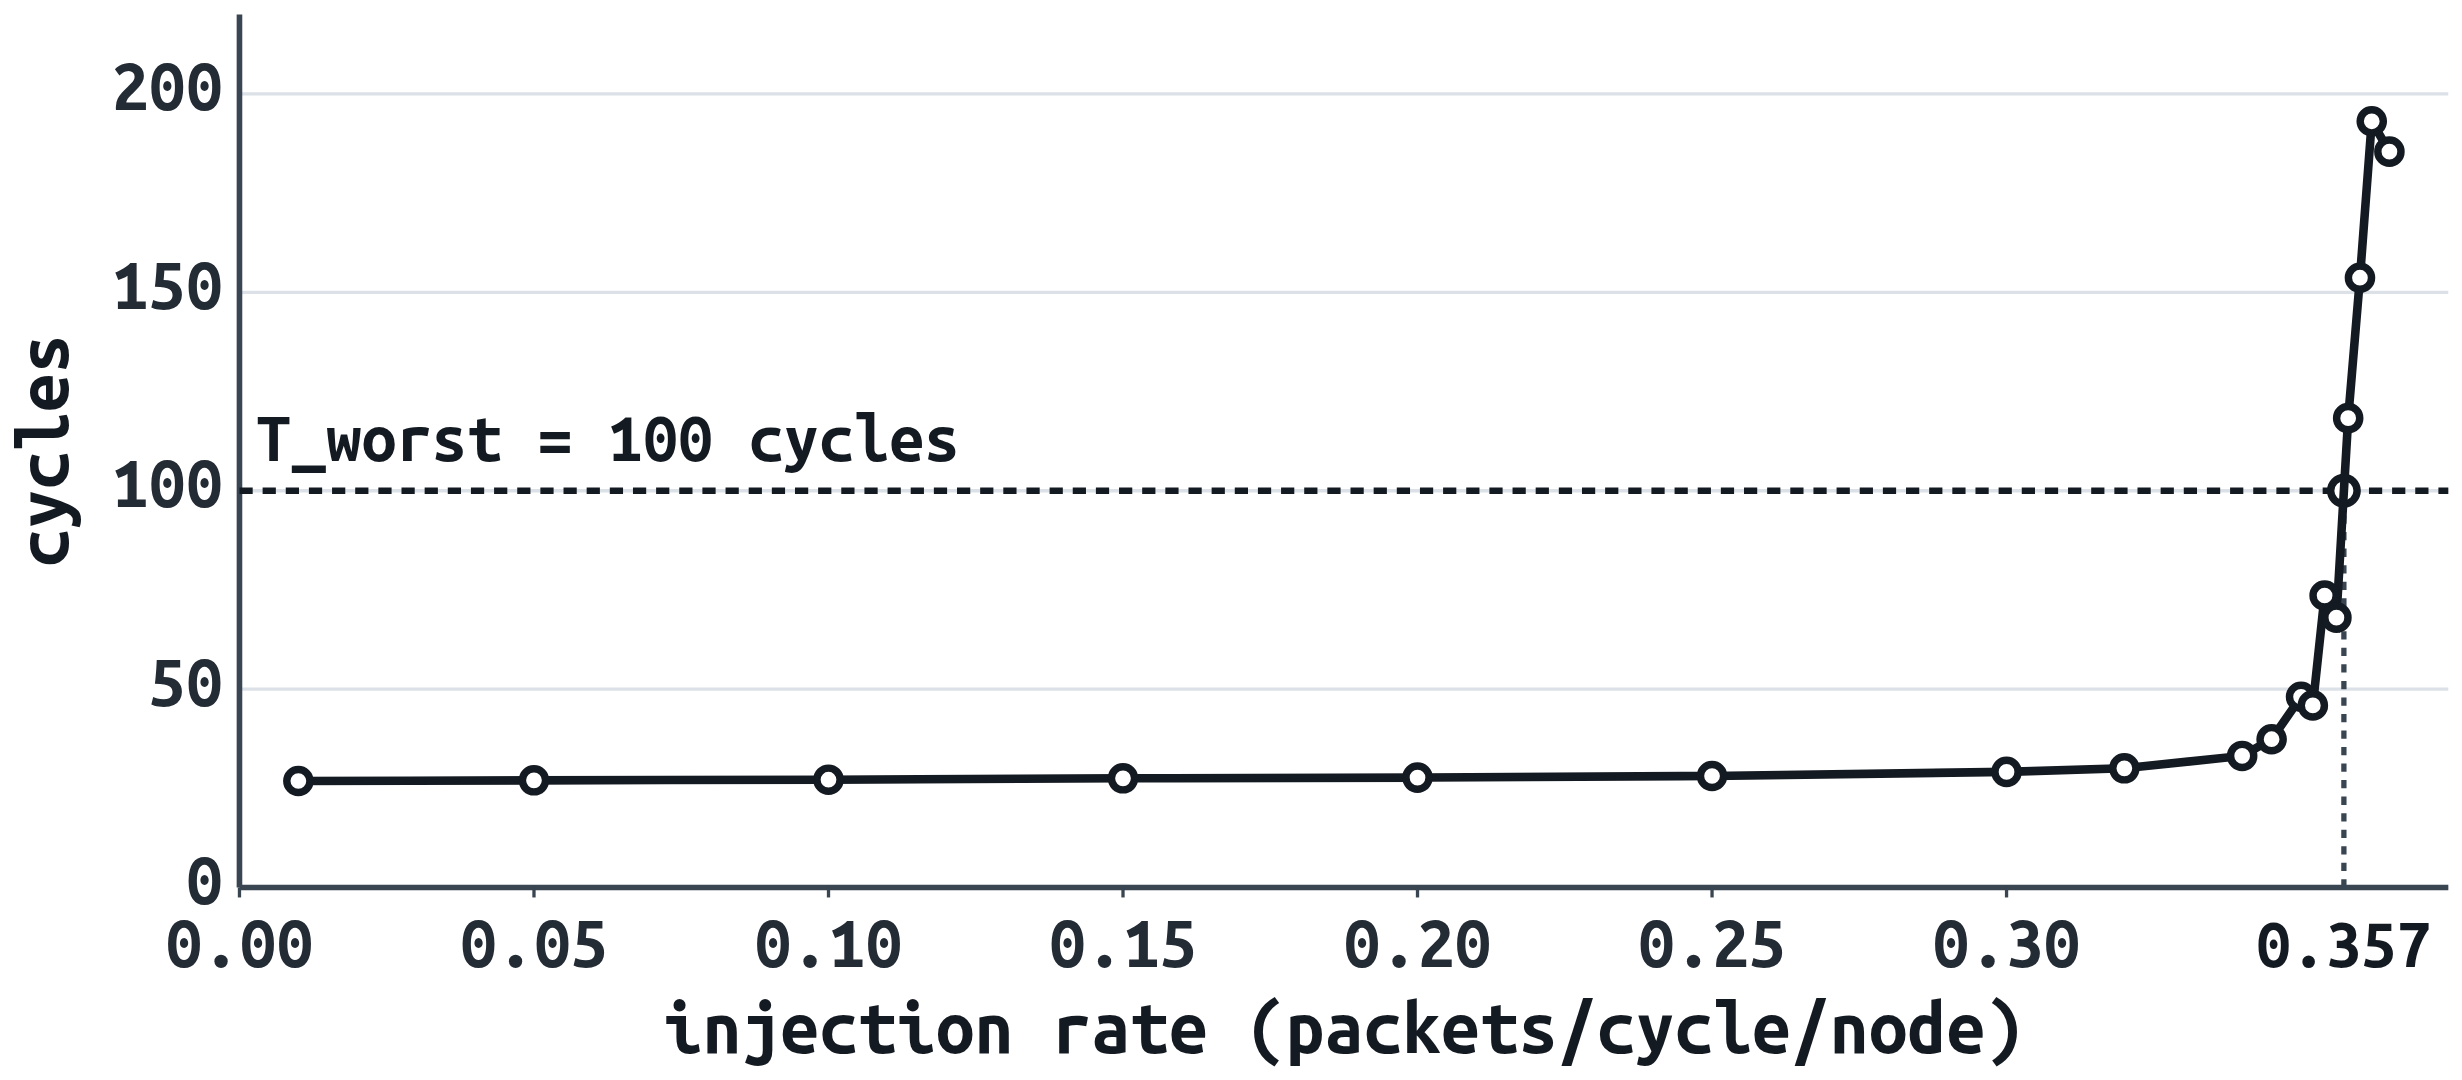
\includegraphics[width=0.95\columnwidth]{figs_new/boundnoc_worst_case_booksim.png}
    %{figs/worst-case-simulation-8x8.pdf}
    \caption{Average network latency of the worst-case (transpose) traffic pattern in an $8\times8$ mesh topology simulated using Booksim~\cite{booksim}.
    The network saturates at injection rate~0.357; we set $T_{worst}=100$ cycles to cover the worst-case round-trip latency just before saturation.}
    \label{fig:jitter-threshold}
\end{figure}

For every Security Sensitive request, the source NI sends the packet through the network and records the actual round-trip latency $T_{orig}$ upon receiving the response.
The source NI then buffers the response in a Delay Queue (DQ) for $T_{worst}-T_{orig}$ cycles before forwarding it to the core.
Thus, \jscheme{} makes every LLC-hit round-trip latency equal to $T_{worst}$, preventing any NUCA timing attack.

\begin{figure}[t]
    \centering
    \includegraphics[width=0.9\linewidth]{figs/NI-updates-v2.pdf}
    \caption{Network Interface extended with a Delay Queue (DQ) and arbitrator (ARB) for \jscheme{}.}
    \label{fig:ni_update}
\end{figure}

\jscheme{} requires minimal hardware changes, as shown in Figure~\ref{fig:ni_update}.
The existing stall queues of the NIs can serve as Delay Queues (DQs) with the addition of multiplexers and an arbitrator (ARB).
Delay is applied only to responses corresponding to LLC hits.
When the destination bank determines that a request causes an LLC miss, it marks the response with a \emph{Delay Required} flag set to \emph{False}.
The source NI skips the delay for such responses and forwards them immediately.

Although \jscheme{} is simple and intuitive, it incurs significant performance overhead because every Security Sensitive LLC-hit access suffers the worst-case latency.
As multicores grow larger, $T_{worst}$ may reach hundreds of cycles, further exacerbating this overhead.
We therefore propose \bscheme{} to reduce this cost.

\subsection{\bscheme} \label{sec-bscheme}
\bscheme{} uses a combination of delay and bypass to achieve both security and performance.
Its goal is to reduce the target round-trip latency from $T_{worst}$ to a lower value $T_{low}$, defined as:
\begin{equation}
\label{eq:tlow}
T_{low} = T_{src \to CHA}^{worst} +
          T_{CHA \to dest}^{worst} +
          T_{dest \to src}^{bypass}
\end{equation}
where $T_{src \to CHA}^{worst}$ and $T_{CHA \to dest}^{worst}$ are the worst-case one-way latencies for those legs, and $T_{dest \to src}^{bypass}$ is the minimum achievable latency from the furthest destination back to the source using router bypass.
We assume the worst case for the first two legs since the attacker controls the source and the requested address, which determines the CHA location.
We choose to expedite only the destination-to-source leg because it carries the actual data, and doing so alone is sufficient to eliminate runtime overhead.

Packets from far destination NIs use bypass to meet $T_{low}$, while packets from nearby NIs use delay.
Algorithm~\ref{alg:defense} details the per-packet decisions made at the source and destination NIs.
Based on the expected round-trip latency $EL_P$~\cite{xiang2016model}, \bscheme{} decides whether to use the bypass channel or regular routing.
If $EL_P > T_{low}$ (Line~11), bypass is used for the response packet.
After the response arrives at the source NI, \bscheme{} checks whether it arrived earlier than $T_{low}$ (Line~17) and adds any remaining delay as needed.

\begin{algorithm}[t]
\footnotesize
\KwData{Sensitive Packet P}
    Src $\leftarrow$ Source NI of the sensitive instruction\;
    Dest $\leftarrow$ Destination NI of the sensitive instruction\;
    $T_{low}$ $\leftarrow$ Target round-trip latency (Equation~\ref{eq:tlow})\;
    $EL_P$ $\leftarrow$ Expected round-trip latency of P from Src to Dest\;
    \If{P is a request packet}{
        Use normal routing protocol for P\;
    }\Else{
        \tcp{P is a response packet from Dest}
        \If{Current NI $=$ Dest}{
            \eIf{$EL_P > T_{low}$}{
                Use bypass for P from Dest to Src\;
            }{
                Use normal routing protocol for P\;
            }
        }\ElseIf{Current NI $=$ Src}{
            $AL_P$ $\leftarrow$ Actual round-trip latency from Src to Dest\;
            \If{$AL_P < T_{low}$}{
                Delay P for $T_{low} - AL_P$ cycles\;
            }
        }
    }
\caption{\bscheme{} packet handling at the NI.}
\label{alg:defense}
\end{algorithm}

To implement bypass, \bscheme{} does not require new physical links.
Instead, one flit-sized buffer is reserved at every router along the bypass path to ensure space for bypassed flits.
This can be extended to support multiple simultaneous flits when multiple NUCA timing attacks occur concurrently.

\bscheme{} also handles congestion-based attacks.
When the source router experiences congestion, it may be unable to forward bypass packets in time.
To detect congestion early, \bscheme{} monitors the credit flow from downstream routers, which indicates the number of free buffers available~\cite{dally1993deadlock,kim2005low,gratz2008regional}.
If no credits are received from a downstream router within a threshold time $T_{cong}$, congestion is assumed on that path.
Upon detecting congestion, \bscheme{} switches from static XY routing to adaptive routing~\cite{duato2001general,gratz2008regional,kim2005low} to avoid the congested path, and combines adaptive routing with bypass to ensure packet delivery within $T_{low}$.


\section{Implementation Details}
\label{sec:impl}
In this section, we describe the design choices made to implement \scheme{} hardware.

\subsection{Changes in the Network Interface} \label{sec-ni-changes}
We extend the Network Interface (NI) to control the timing of packet ejection, which is central to the defense mechanism of \scheme{}.
NI extensions have previously been used to provide security features such as malware detection~\cite{novo2020flow} and network intrusion detection~\cite{mirsky2018kitsune}.
We extend NI capability to detect packets that require delay or bypass based on their expected latency, following the \scheme{} logic described in Section~\ref{sec-overview}.

When the NI receives a load request, it sets flags to decide between the two available networks (normal or bypass) or to add delay (for \jscheme{}).
The bypass network uses the same physical links as the normal network.
We use virtual channel (VC) separation to isolate bypass traffic from regular network traffic~\cite{duato2001general}.
Bypass packets use a dedicated VC, ensuring that bypass traffic does not interfere with normal network operation.

The NI uses a 1-bit flag \texttt{bypass\_flag} on each output port of the router.
When the NI sends any flit through an output port, it checks whether \texttt{bypass\_flag} is enabled for that cycle.
If the flag is disabled, the NI cannot send the flit on that cycle.
When \bscheme{} needs to send a flit via the bypass path, the NI first checks and sets this flag.
If the flag is already set, the NI stalls the flit and retries on subsequent cycles.

In the common case, the attacker targets only two distinct LLC banks.
Since XY routing produces non-overlapping bypass paths for different source-destination pairs in a mesh, bypass contention is unlikely in practice.
However, collisions can be resolved by pipelining the bypass mechanism.

When an NI sends a flit through either the bypass or regular path, it sets a timestamp in the header flit.
For request flits, the timestamp records the flit creation time.
For response flits, the timestamp records the creation time of the corresponding request flit.
This timestamp is used by the \scheme{} logic in the NI.
\scheme{} uses a comparator and multiplexer (MUX) in the NI to implement the defense.
Figure~\ref{fig:block-diagram} illustrates the bypass operation using the existing NI buffers.

\begin{figure}[t]
\centering
\includegraphics[width=\linewidth]{figs/NI Block Diagram 2.pdf}
\caption{Block diagram of bypass operations in the extended Network Interface.}
\label{fig:block-diagram}
\end{figure}

\subsection{Delay Implementation} \label{sub:jitter}
To implement dynamic delay, each NI includes a Delay Queue (DQ) that buffers flits associated with Security Sensitive instructions until their target latency is met.
Every flit carries a Target Latency (TL) field in its header, set to $T_{worst}$ (\jscheme{}), $T_{low}$ (\bscheme{}), or a pseudorandomly drawn $T_{rand}$ (\rscheme{}) based on the defense scheme in use.

For \rscheme{}, $T_{rand}$ is derived rather than stored.
Both the destination NI and the source NI compute $T_{rand}$ independently, using a pseudorandom function of the timestamp already carried in the flit header (Section~\ref{sec-ni-changes}).
Both NIs apply the same function with the same seed to the same timestamp, so they compute the identical value.
No extra communication or storage is needed beyond the existing timestamp field.

When the tail flit of a Security Sensitive response arrives at the source NI, the NI computes the Round-Trip Latency (RTL) of the request using the stored timestamp and compares it to TL using a comparator.
There are two cases:
\begin{compactenum}
    \item \textbf{RTL $\geq$ TL:} No delay is needed.
    The flit is forwarded to the ejection queue of the NI immediately, or placed in the stall queue if the ejection queue is unavailable.

    \item \textbf{RTL $<$ TL:} The flit is placed in the DQ at the source NI with a delay of $TL - RTL$ cycles.
    A counter wakes up the NI to eject the flit after the specified delay has elapsed.
\end{compactenum}


%\section{Discussion}
%\label{sec:discuss}
%\input{discussion}
\section{Security Analysis}
\label{sec:security}
In this section, we provide a security analysis of the effectiveness and robustness of \scheme{}.
We define security in this context as follows: \scheme{} succeeds if an attacker cannot distinguish, with non-negligible advantage, between a Security Sensitive access to a near-tile LLC bank and one to a far-tile LLC bank based on observed latency.

\begin{figure*}[t]
    \centering
    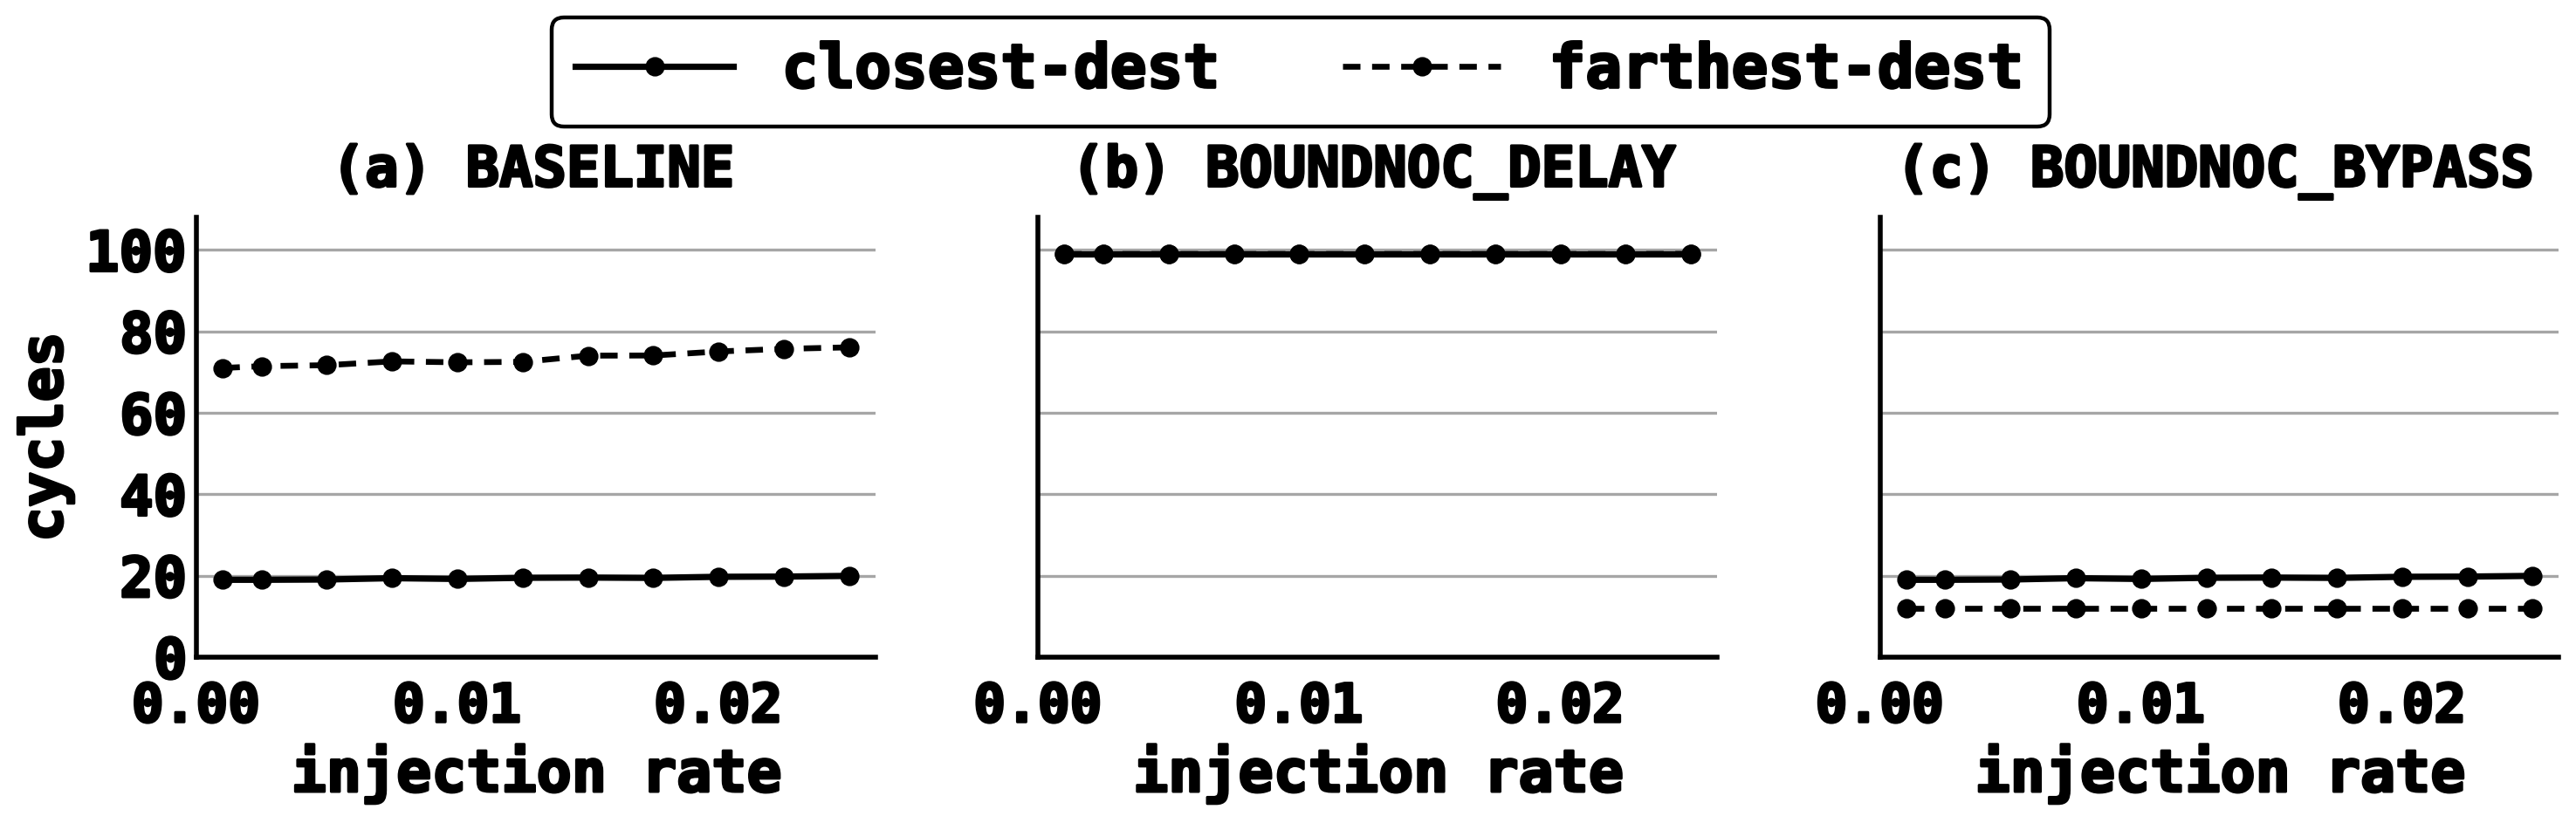
\includegraphics[width=0.85\linewidth]{figs_new/boundnoc_roundtrip_latency_syn.png}
    %{figs/attack-packet.pdf}
    \caption{Impact of different policies on Secure Load round-trip latency for a synthetic workload.
    (a)~\basescheme{}: near-tile and far-tile latencies are clearly separable.
    (b)~\jscheme{}: latencies are indistinguishable but elevated.
    (c)~\bscheme{}: latencies are indistinguishable with near-optimal absolute latency.}
    \label{fig:impact-on-latency-syn}
\end{figure*}

\subsection{\jscheme} \label{sec-security-jscheme}
In \jscheme{}, the timing difference between a nearby LLC access and a faraway LLC access is mitigated by adding delays to sensitive LLC accesses at the source NI.
The LLC access latency in \cpumodel{} consists of two parts: the latency to the CHA, and the latency to the LLC slice storing the cache line.
Since the latter depends on which core brought the cache line into the LLC and is unlikely to exhibit observable patterns to the attacker, our main mitigation target is the latency to the CHA, which is determined by the physical address via a hash function.
To eliminate observable patterns, \jscheme{} makes every LLC-hit access a constant-time operation regardless of distance.

We evaluate \jscheme{} by comparing the round-trip latency of far-tile and near-tile cache line accesses at various injection rates.
As shown in Figure~\ref{fig:impact-on-latency-syn}(b), the round-trip latency of a Security Sensitive load with \jscheme{} shows no difference based on distance at injection rates from 0.000 to 0.357.
Note that \jscheme{} provides this guarantee only until the NoC becomes saturated.
Under saturation, LLC latency far exceeds the average and becomes non-deterministic, making it impossible for an attacker to extract reliable distance-based patterns.
We observe that the network saturates at injection rate 0.357, where the round-trip latency does not exceed $T_{worst}=100$ cycles.
Therefore, 100 cycles is a safe delay threshold for \jscheme{}.

\subsection{\bscheme} \label{sec-security-bscheme}
In \bscheme{}, the timing difference is mitigated by enforcing a lower target latency $T_{low}$, defined in Equation~\ref{eq:tlow}, rather than $T_{worst}$.
$T_{low}$ combines the worst-case latency from the source to the CHA, the worst-case latency from the CHA to the destination, and the minimum achievable latency from the destination back to the source using bypass.
For a Security Sensitive packet $p$, there are three scenarios:

\begin{compactenum}[(1)]
    \item The expected round-trip latency without bypass (${EL}_{p}$) is at most $T_{low}$.
    No bypass is needed; \bscheme{} delivers the packet after adding delay to match $T_{low}$.

    \item ${EL}_{p}$ exceeds $T_{low}$, but after applying bypass the actual round-trip latency falls below $T_{low}$.
    This is the common case: \bscheme{} uses router bypass to expedite delivery of $p$ and then adds delay to match $T_{low}$.

    \item ${EL}_{p}$ exceeds $T_{low}$ and the round-trip latency remains above $T_{low}$ even after bypass, which occurs only under network saturation.
    In this case, the observed latency is dominated by non-deterministic congestion rather than distance-dependent LLC access patterns, so an attacker cannot reliably distinguish near-tile from far-tile accesses.
\end{compactenum}

Figure~\ref{fig:impact-on-latency-syn}(c) shows the round-trip latency of a Security Sensitive load with \bscheme{}, confirming no observable difference based on distance at injection rates 0.000 to 0.357.

\subsection{Defense Against Congestion-Based Attacks}
\scheme{} defends against congestion-based attacks by ensuring all Security Sensitive packets are delivered within $T_{low}$, regardless of network congestion.
Since the observed latency is always $T_{low}$, an attacker cannot infer whether the traffic by the victim created congestion on any particular network path.

\subsection{Resistance to Bypass Contention Channel}
Although an attacker could in principle attempt to use the bypass mechanism as a contention channel, \bscheme{} provides no exploitable signal through this channel.
Bypass is applied deterministically based on expected latency rather than on any secret-dependent condition, so bypass usage reveals nothing about the memory access pattern of the victim.
Furthermore, \bscheme{} applies bypass indiscriminately whenever $EL_p > T_{low}$, so the attacker cannot infer contention based on whether bypass is used.
In our experiments (Section~\ref{sec:eval}), the maximum wait time to acquire the bypass path is 2 cycles under non-saturated network conditions, keeping the latency bound tight and predictable.



\section{Evaluation}
\label{sec:eval}
We present the experiments and results used to evaluate \scheme{} in this section.

\subsection{Experimental Setup} \label{sec:eval-setup}
We conducted three sets of experiments.
First, we evaluated the impact of \jscheme{} and \bscheme{} on average packet network latency with varying injection rates using the Garnet~\cite{agarwal2009garnet} simulator.
Second, we measured the performance overhead of both schemes on real applications from the PARSEC~\cite{bienia2008parsec} and Rodinia~v3.0~\cite{che2009rodinia} benchmark suites using the Gem5~\cite{binkert2011gem5} simulator.
Finally, we conducted sensitivity studies to identify optimal design parameters.

We evaluated five policies summarized in Table~\ref{tab:policies}.
All performance results are normalized to \basescheme{} (the insecure baseline without bypass).
When comparing against \basebscheme{}, we state so explicitly.
We used a 64-core machine modeled as an $8\times8$ 2D mesh with a 32~kB L1 cache per core and a 2~MB distributed LLC.
For Rodinia applications, we executed 1B instructions in the region of interest where threads are spawned by the OpenMP library.
For PARSEC applications, we executed 1B instructions or until the end of the marked region of interest.
We treat all load requests arriving at the LLC as Security Sensitive instructions to model the worst-case overhead of \scheme{}.

\begin{table}[t]
    \centering
    \begin{tabular}{|p{0.3\linewidth}|p{0.6\linewidth}|}
        \hline \hline
        \textbf{Policy} & \textbf{Description} 
        \\ \hline
        \basescheme{} 
        & Insecure $8\times8$ 2D mesh baseline 
        \\ \hline
        \basebscheme{} 
        & Bypass network on top of \basescheme{} following~\cite{perez2019smart++}, without security enforcement \\ 
        \hline
        \jscheme{} 
        & \basescheme{} extended with a delay queue at each NI; delays all Security Sensitive LLC hits to $T_{worst}$ \\ 
        \hline
        \bscheme{} 
        & \basescheme{} extended with bypass and delay; enforces $T_{low}$ for all Security Sensitive LLC hits \\ 
        \hline
        \rscheme{}
        & \basescheme{} extended with bypass and delay; draws a random target from $[T_{floor}, T_{low}]$ per access instead of enforcing the fixed $T_{low}$ \\
        \hline
    \end{tabular}
    \caption{The five evaluated policies. 
    All results are normalized to \basescheme{}.}
    \label{tab:policies}
\end{table}

\subsection{Average Packet Network Latency} \label{sec:avg-latency}
We used the Garnet simulator to measure average packet latency at varying injection rates.
Figure~\ref{fig:overall_packet_network_latency} shows the results.
\bscheme{} performs comparably to \basescheme{} across all injection rates: using bypass paths for Security Sensitive loads does not adversely affect overall average packet latency.
In contrast, \jscheme{} causes the network to saturate earlier than \basescheme{} at higher injection rates, due to the delay queue increasing congestion in the network.

\basebscheme{} and \bscheme{} are visually identical in this figure: bypass alone already meets the target latency, so the delay-convergence check has nothing left to do.
\jscheme{} and \basescheme{} converge too, but only past the saturation knee, once padding no longer fires.
Below saturation the two remain distinguishable, just not at a scale visible on this axis.

\begin{figure}[t]
    \centering
    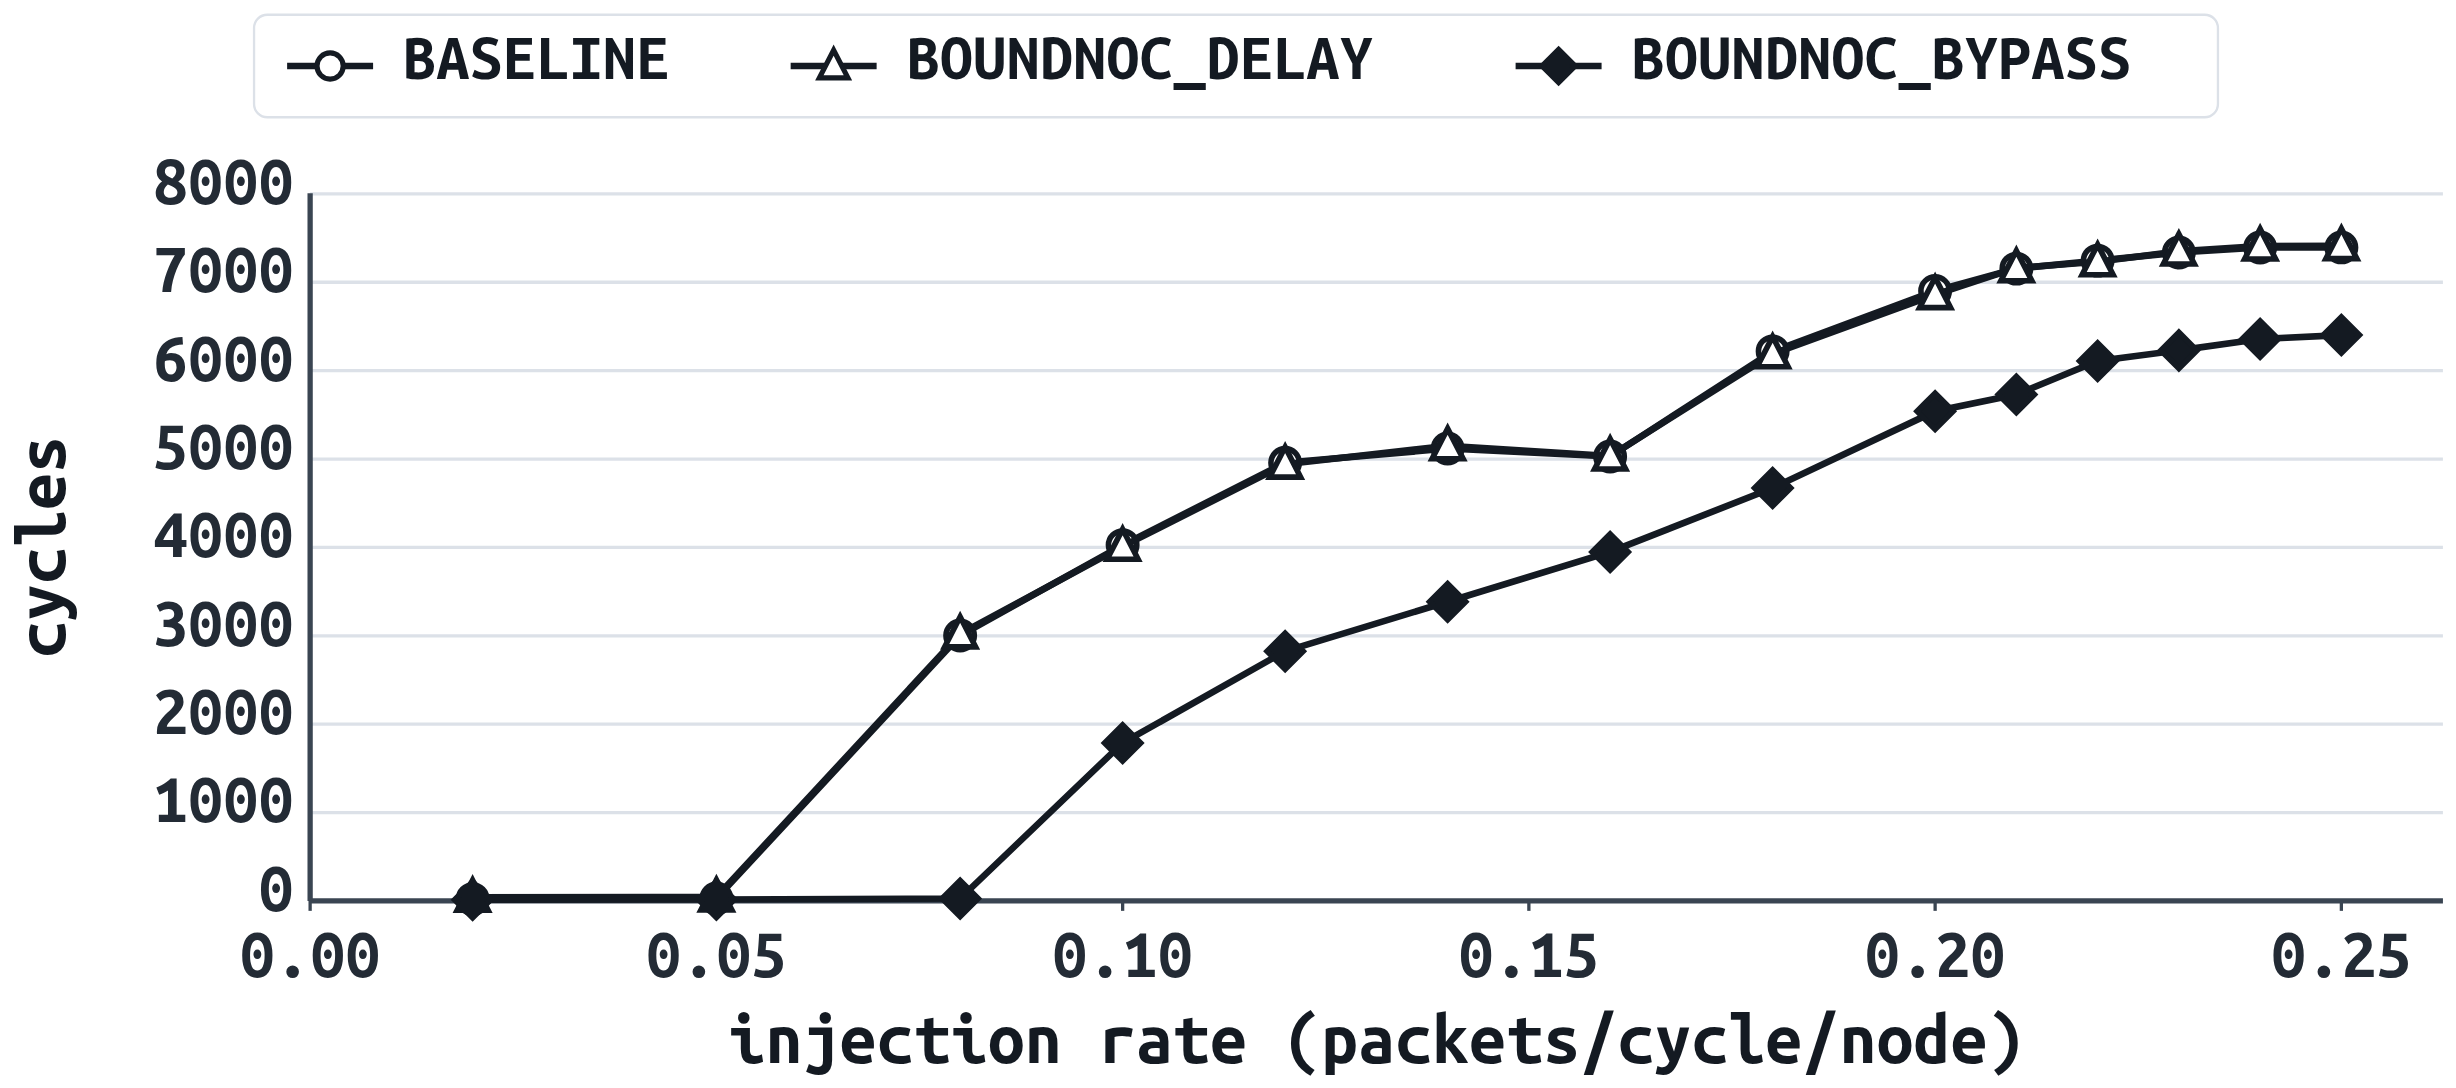
\includegraphics[width=\linewidth]{figs_new/boundnoc_injection_rate_sweep.png}
    %{figs/overall_packet_network_latency.pdf}
    \caption{Average packet latency vs.\ injection rate for \basescheme{}, \basebscheme{}, \jscheme{}, and \bscheme{}, using uniform-random synthetic traffic on an $8\times8$ mesh (Garnet\_standalone).}
    \label{fig:overall_packet_network_latency}
\end{figure}

\subsection{Impact on Secure Load Latency} \label{sec:secure-ld-latency}
We evaluate the impact of each policy on the round-trip latency of Security Sensitive loads using both synthetic and real workloads.

\subsubsection{Synthetic Workload} 
Figure~\ref{fig:impact-on-latency-syn} shows the round-trip latency of Security Sensitive loads at varying injection rates using the Garnet simulator.
In the baseline, near-tile and far-tile accesses are clearly distinguishable.
Both \jscheme{} and \bscheme{} eliminate this distinction, making near- and far-tile latencies indistinguishable from the the perspective of the attacker.
However, \jscheme{} incurs a significantly higher absolute latency than \bscheme{}, since all accesses are delayed to $T_{worst}$ rather than $T_{low}$.

\subsubsection{Real Workload}
Figure~\ref{fig:impact-on-latency} (\S\ref{sec-security-real}) confirms that \jscheme{} and \bscheme{} both produce overlapping latency distributions for the closest and farthest node pairs on leukocyte, a real application.

\subsection{Performance Overhead} \label{sec:perf-overhead}

\begin{figure*}[t]
\centering
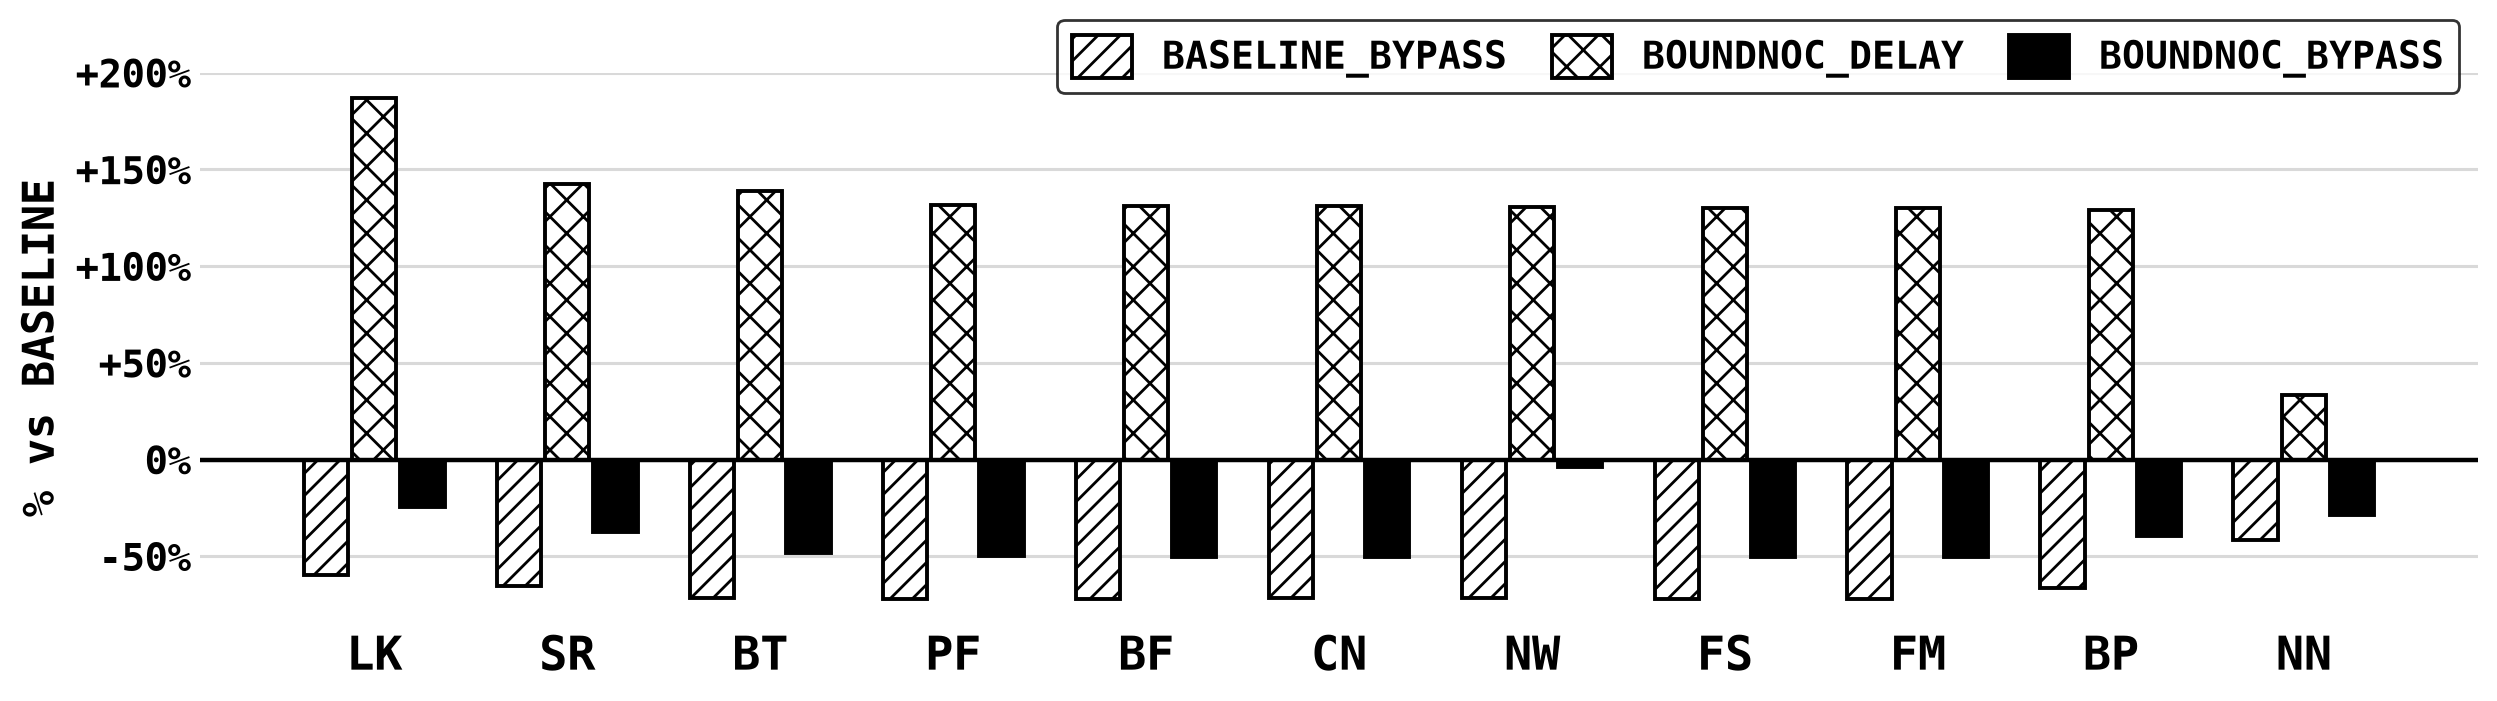
\includegraphics[width=\linewidth]{figs_new/boundnoc_latency_pctdelta.png}
%{figs/performance-overhead.pdf}
\caption{Performance overhead of \jscheme{} and \bscheme{} on PARSEC~\cite{bienia2008parsec} and Rodinia~\cite{che2009rodinia} benchmarks, normalized to \basescheme{}.
Shorthand described in the Appendix.}
\label{fig:performance-overhead}
\end{figure*}

Figure~\ref{fig:performance-overhead} shows the performance overhead of all four policies.
\jscheme{} incurs $0.53\%$--$15.0\%$ overhead over \basescheme{}, with a geomean of $7.24\%$ across all applications.
Compared to the insecure \basebscheme{}, \jscheme{} overhead is $11.94\%$ and \bscheme{} overhead is $1.96\%$.

Figure~\ref{fig:bypass-count} shows that the bypass packet count of \bscheme{} matches that of \basebscheme{} closely in every benchmark, differing by at most $2\%$.
\bscheme{} uses the same bypass decision as \basebscheme{}; the only added cost is the delay needed to pad each response up to $T_{low}$.
This is why the overhead of \bscheme{} over \basebscheme{} stays small ($1.96\%$ geomean) across every application we tested.

\begin{figure*}[t]
\centering
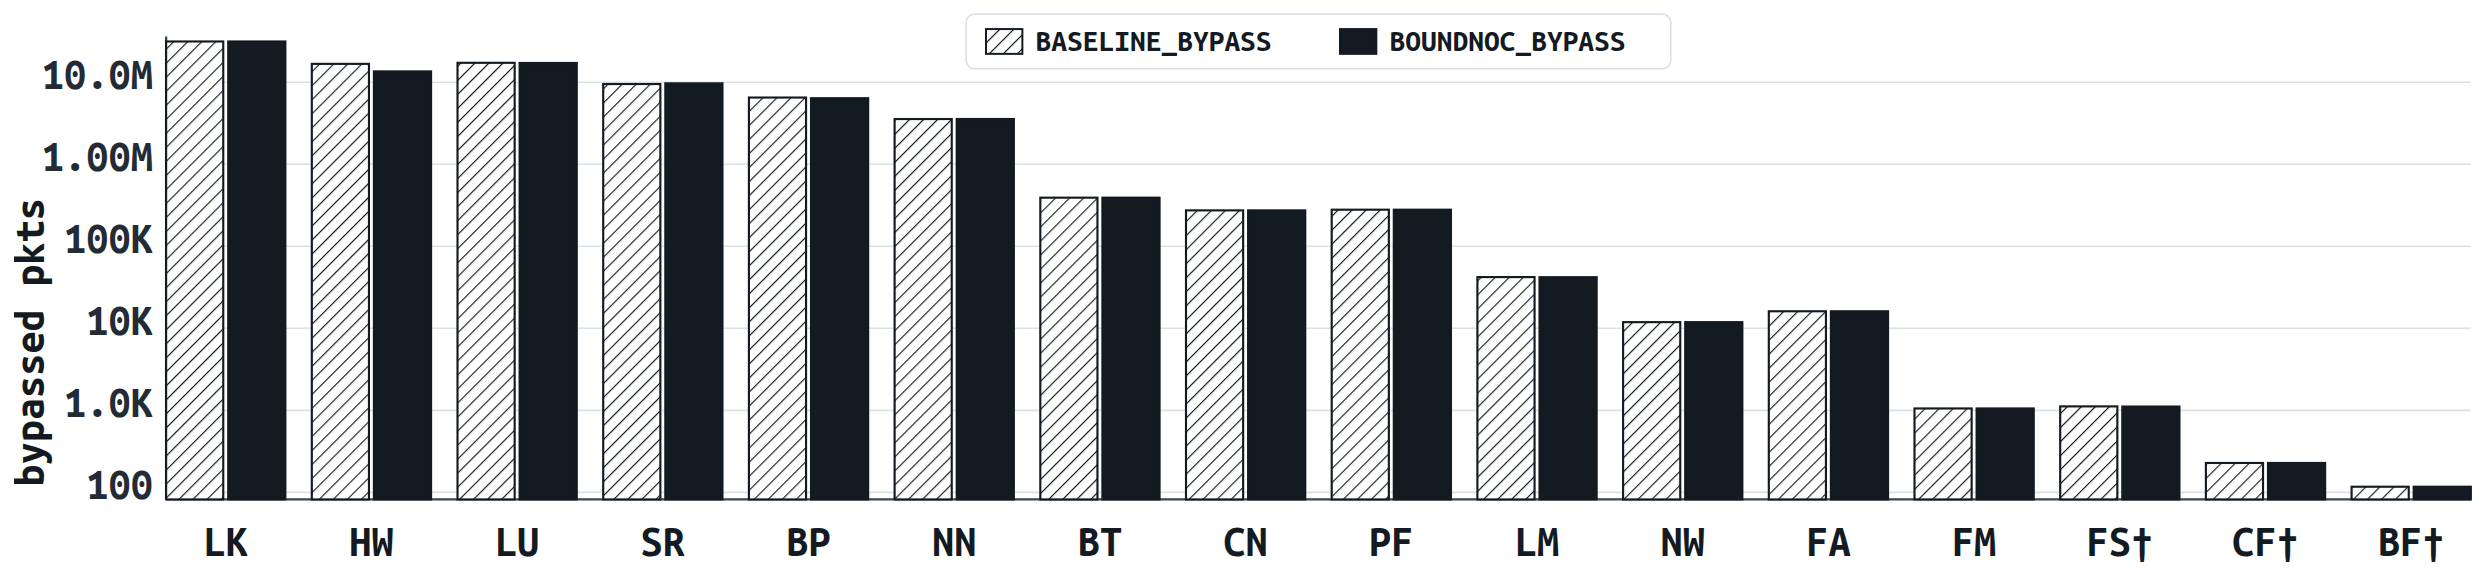
\includegraphics[width=\linewidth]{figs_new/boundnoc_bypass_count.png}
%{figs/bypass-count.pdf}
\caption{Total bypass packet count for \basebscheme{} and \bscheme{} using PARSEC~\cite{bienia2008parsec} and Rodinia~\cite{che2009rodinia} benchmarks.}
\label{fig:bypass-count}
\end{figure*}

%In some applications, \bscheme{} does not improve over \basescheme{}.
%For example, x264 incurs $4\%$ overhead under \bscheme{}.
%In x264, \bscheme{} causes certain threads to execute more instructions before the 1B-instruction termination condition is met on any thread, increasing the measured execution time relative to baseline.

\subsection{Impact on Delay Amount} \label{sec:delay-amount}
Figure~\ref{fig:delay-amount} shows the total delay cycles accumulated in the delay queue for PARSEC applications.
\jscheme{} forces all Security Sensitive packets to wait in the delay queue until $T_{worst}$, resulting in high total delay.
\bscheme{} delays only packets that arrive earlier than $T_{low}$, substantially reducing total delay cycles and the associated performance overhead.

\begin{figure*}
    \centering
    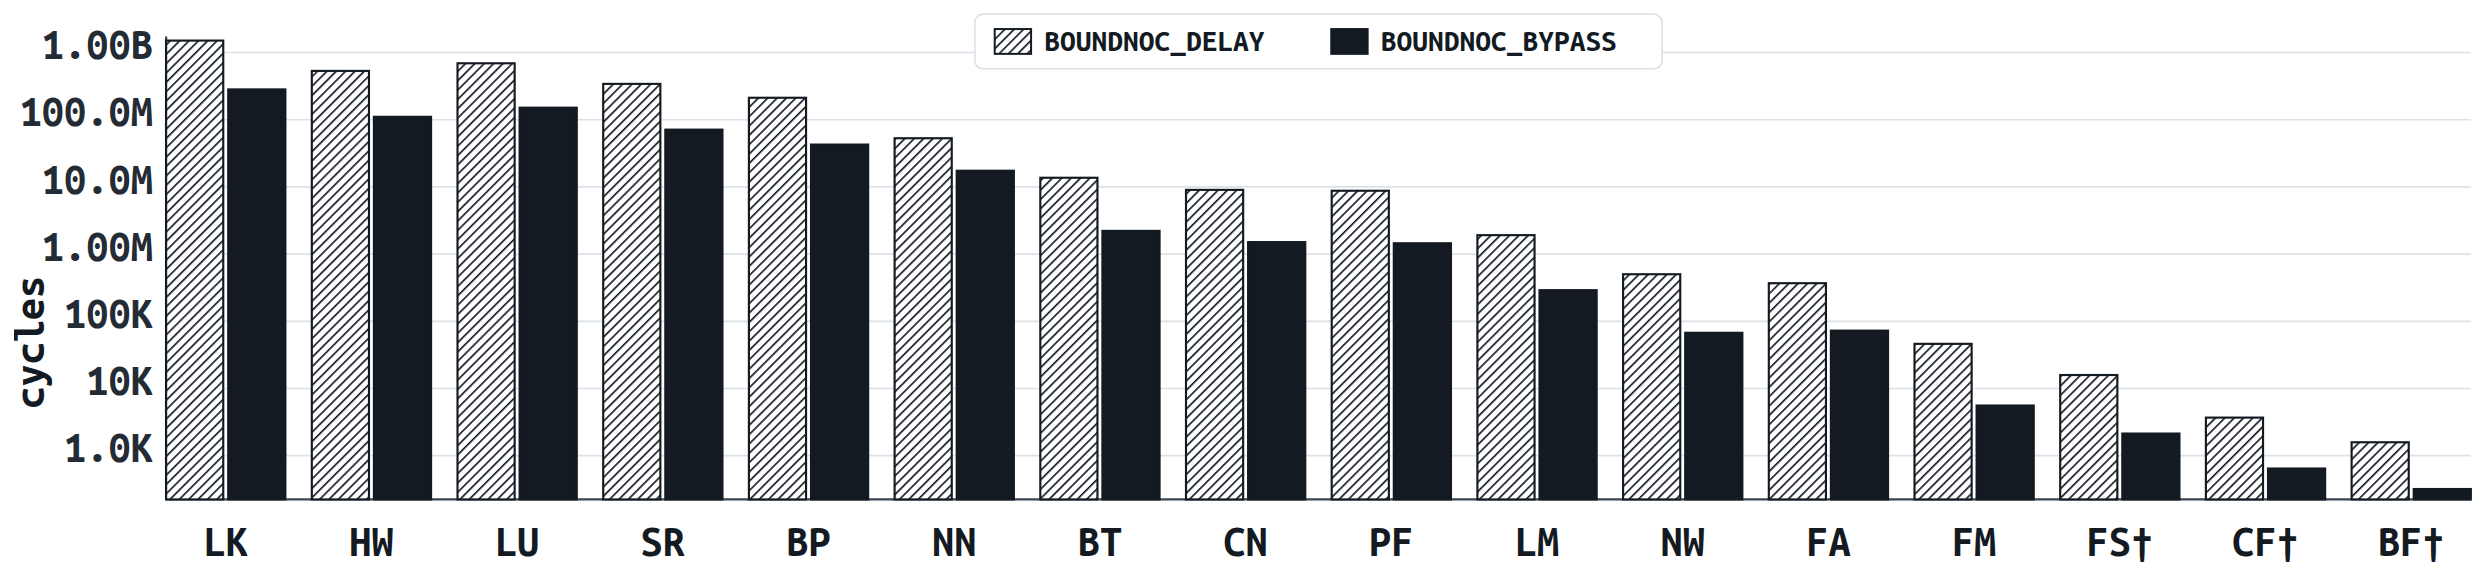
\includegraphics[width=\linewidth]{figs_new/boundnoc_delay_amount.png}
    %{figs/delay-amount.pdf}
    \caption{Total delay cycles accumulated in the delay queue for PARSEC applications under \jscheme{} and \bscheme{}.}
    \label{fig:delay-amount}
\end{figure*}

\subsection{MLPerf Overheads} \label{sec:mlperf}
We present the overheads of \jscheme{} and \bscheme{} on MLPerf TinyML~\cite{banbury2021mlperf} workloads in Figure~\ref{fig:impact-on-mlperf}.

\begin{figure}[t]
   \centering
    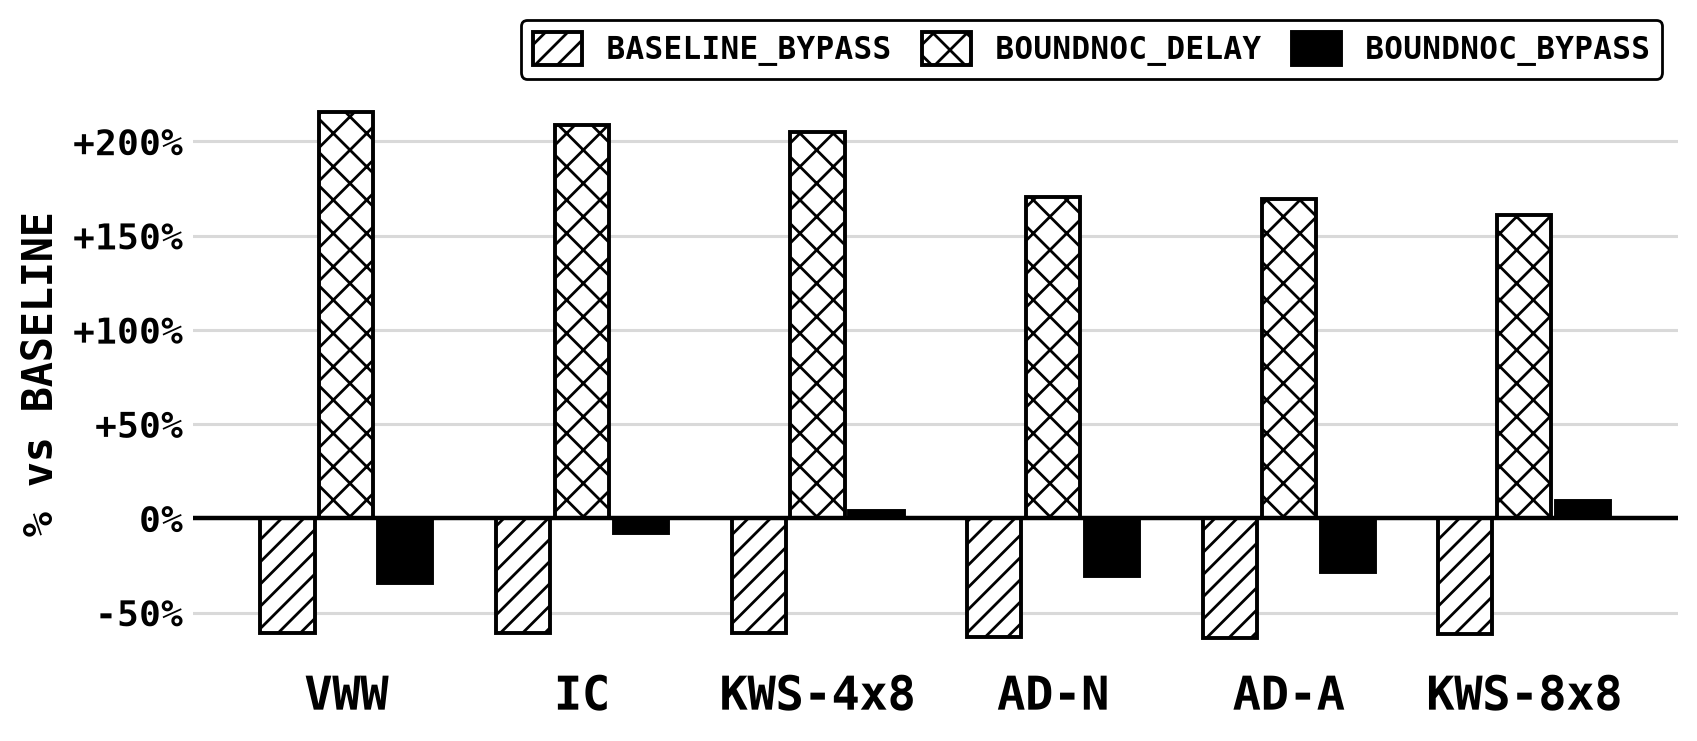
\includegraphics[width=\linewidth]{figs_new/boundnoc_ml_latency_pctdelta.png}
    %{figs/impact-on-latency.pdf}
    \caption{Mean attack-packet latency under \basebscheme{}, \jscheme{}, and \bscheme{}, expressed as \% change relative to \basescheme{}, for four MLPerf TinyML inference workloads. 
    KWS is shown at both a $4\times8$ and an $8\times8$ mesh to isolate topology effects; AD is shown for both its AD-N and AD-A input classes.}
    \label{fig:impact-on-mlperf}
\end{figure}

We evaluate four TinyML inference workloads from the MLPerf TinyML suite: Anomaly Detection (AD), Keyword Spotting (KWS), Image Classification (IC), and Visual Wake Words (VWW).
Each workload is a fully int8-quantized TensorFlow Lite Micro model, compiled into a statically-linked musl binary and executed natively on each simulated core.
No host-side interpretation or instrumentation is introduced into the timing loop.

AD uses a $270$~KB fully-connected deep autoencoder~\cite{autoencoder} over a 5-frame, 128-band log-mel spectrogram ($5\times128$) derived from the ToyADMOS industrial-sound dataset~\cite{koizumi2019toyadmos} to perform unsupervised anomaly detection.
It completes with $2.9$~million instructions per core. 
We evaluate both a \emph{normal} (AD-N --- a recording of the ToyCar operating normally) and an \emph{anomalous} (AD-A --- containing an injected mechanical fault) input clip, replicated across 64 independent instances on an $8\times8$ mesh.

KWS performs small-vocabulary keyword spotting with a $52.5$~KB depthwise-separable CNN (DS-CNN)~\cite{zhang2017hello} over a $49\times10$ MFCC feature matrix extracted from the Google Speech Commands dataset~\cite{warden2018speech}. 
It completes with $204$~million instructions per core -- an order of magnitude more compute-intensive than AD.
Because of this cost, we evaluate KWS at both a $4\times8$ mesh (32 instances, KWS-4x8) and the standard $8\times8$ mesh (64 instances, KWS-8x8) to separate topology effects from workload effects.

IC performs 10-class image classification with a $96$~KB ResNet8~\cite{he2016resnet} model over $32\times32\times3$ CIFAR-10~\cite{krizhevsky2009learning} images. 
It completes with $941$~million instructions per core, replicated across 32 instances on a $4\times8$ mesh.

VWW performs binary person detection with a $325$~KB, width-reduced ($0.25\times$) MobileNetV1~\cite{howard2017mobilenets} model over $96\times96\times3$ crops from the Visual Wake Words dataset~\cite{chowdhery2019vww}. 
It completes with $628$~million instructions per core, also replicated across 32 instances on a $4\times8$ mesh.

As with the Rodinia and PARSEC results in Section~\ref{sec:eval-setup}, we mark memory accesses of every core  as Security Sensitive to model the worst case, and use $T_{low}=50$ and $T_{worst}=100$ cycles for \bscheme{} and \jscheme{} respectively.
Because AD, IC, and VWW are single-threaded inference binaries, we replicate an independent instance to every core rather than let 63 cores sit idle waiting on a single active thread.

Figure~\ref{fig:impact-on-mlperf} shows the mean attack-packet latency under each policy, expressed as percentage change relative to \basescheme{}.
Across all six workload/mesh combinations, \basebscheme{} reduces mean attack-packet latency by $60\%$--$63\%$ and \jscheme{} increases it by $161\%$--$216\%$, consistent with the Rodinia/PARSEC results in Section~\ref{sec:perf-overhead}. 
\jscheme{} enforces the fixed worst-case latency $T_{worst}$ for every Security Sensitive access regardless of workload, while \basebscheme{} is bounded only by how much traffic the bypass path can absorb.

\bscheme{} shows a workload-dependent split not previously visible from Rodinia and PARSEC alone.
On AD-N, AD-A, and VWW, \bscheme{} closely tracks \basebscheme{}, improving over \basescheme{} by $30.5\%$, $28.7\%$, and $34.2\%$ respectively.
On KWS and IC, \bscheme{} instead lands close to or slightly above \basescheme{}: $+9.1\%$ on KWS-8x8, $+4.1\%$ on KWS-4x8, and $-8.0\%$ on IC.
The KWS regression is robust to topology -- it appears at both $4\times8$ and $8\times8$ mesh, ruling out mesh diameter as the sole cause. 
IC reproduces the same weak-to-negative pattern despite running on the same $4\times8$ mesh as VWW, which shows the opposite, favorable result.

We compared the bypass-eligible packet fraction, jittered-packet fraction, and mean hop count across all six runs and found no single aggregate statistic that cleanly separates the two groups.
Bypass-eligible fraction is nearly uniform ($62\%$--$71\%$) across all six. 
Jittered-packet fraction separates AD from KWS at matched $8\times8$ scale ($4.1\%$ vs.\ $18.3\%$) but not IC from VWW at $4\times8$ scale ($98.5\%$ vs.\ $67.3\%$, the wrong direction).
Mean hop count tracks mesh geometry rather than the workload grouping.

We conclude that the hop-count-based bypass eligibility threshold for \bscheme{} is not uniformly effective across all inference workloads. 
The convolutional, activation-heavy access patterns of KWS and IC appear less amenable to it than the single fully-connected pass of AD or the wider MobileNet of VWW. 
We leave a precise mechanistic explanation to future work; Section~\ref{sec:eval-rand} explores a different mitigation, randomizing the convergence target instead of the eligibility threshold itself.

\subsection{\rscheme{}: A Randomized-Target Alternative} \label{sec:eval-rand}
As a sensitivity study over the randomization window (Section~\ref{sec:eval-setup}), we compare \bscheme{} against two alternative target ranges.
\bscheme{} underperforms on two of the six MLPerf combinations: KWS-4x8 ($+4.1\%$) and KWS-8x8 ($+9.1\%$), with IC only a modest improvement ($-8.0\%$).
This motivates \rscheme{} (Section~\ref{sec-rscheme}), which draws a random target per access instead of the fixed $T_{low}$.

We first tried a wider variant (\rejscheme{}) that draws the target uniformly from $[T_{floor}, T_{worst}]$ instead of $[T_{floor}, T_{low}]$.
This wider range costs too much average latency in practice: it lands worse than \basescheme{} on every benchmark we tested.
We do not use it further.

\rscheme{} instead draws from the narrower $[T_{floor}, T_{low}]$ range.
Figure~\ref{fig:variable-workload} compares \basebscheme{}, \bscheme{}, \rejscheme{}, and \rscheme{} on eight benchmarks spanning MLPerf, PARSEC, and Rodinia.
\rscheme{} fixes both weak MLPerf cases -- IC improves to $-41.0\%$, KWS-4x8 to $-32.5\%$, KWS-8x8 to $-26.3\%$ -- while making the already-strong PARSEC and Rodinia cases stronger still.
\rscheme{} is a clean latency win on every benchmark tested.

\begin{figure*}[t]
\centering
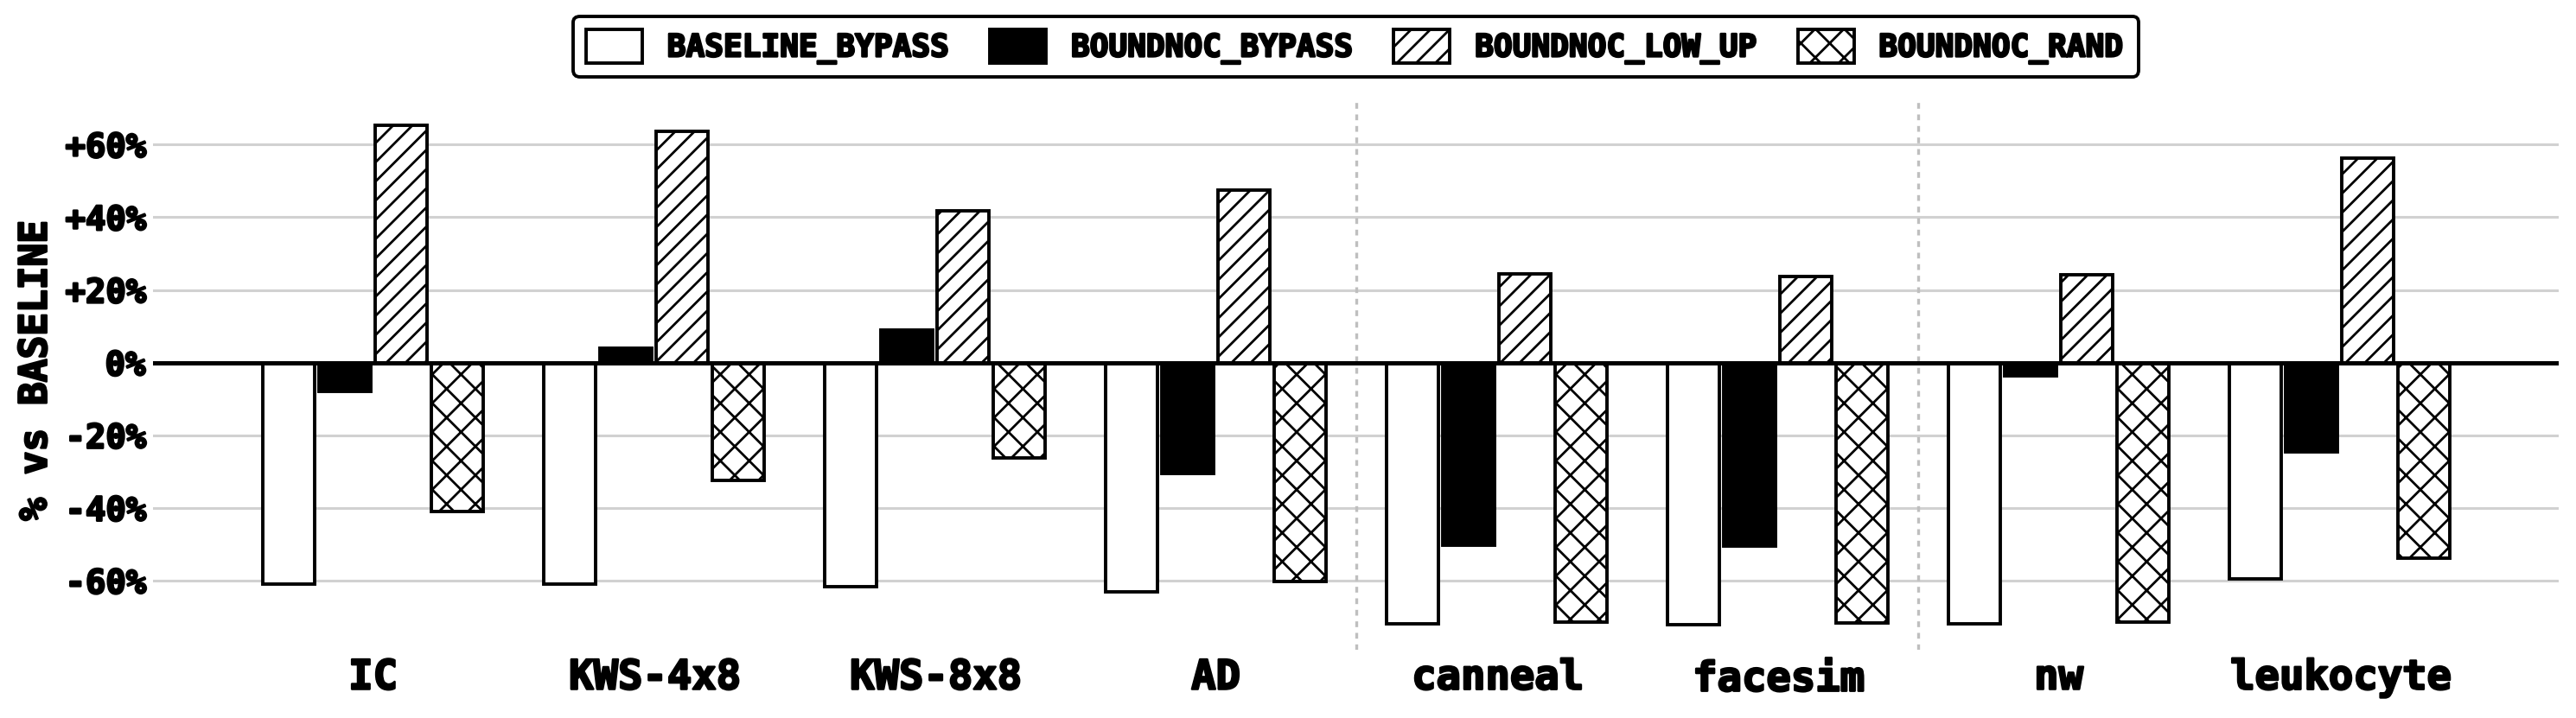
\includegraphics[width=\linewidth]{figs_new/boundnoc_variable_workload_pctdelta.png}
\caption{Mean attack-packet latency under \basebscheme{}, \bscheme{}, \rejscheme{}, and \rscheme{}, expressed as \% change relative to \basescheme{}, across eight benchmarks spanning MLPerf TinyML, PARSEC~\cite{bienia2008parsec}, and Rodinia~\cite{che2009rodinia}.}
\label{fig:variable-workload}
\end{figure*}

This latency benefit does not come with the same security guarantee as \bscheme{}, however.
Section~\ref{sec-security-rand} shows \rscheme{} is less effective than \bscheme{} at hiding distance, though still better than \basebscheme{}.

\subsection{Hardware Overhead} \label{sec:hw-overhead}
We estimate the hardware cost using CACTI-7~\cite{cacti} at 22~nm.
\scheme{} introduces minimal changes to both the NIs and the routers.
NI changes include a delay queue ($0.981~mm^{2}$, $0.028~nJ$/access) and 512 64-bit comparators.
An arbitration unit with two multiplexers is also added, with negligible area cost.
The bypass channel adds $2.34\%$--$4.69\%$ area overhead compared to a conventional NoC~\cite{ma2021latency}.

In summary, \bscheme{} provides the same security guarantees as \jscheme{} while incurring no performance overhead compared to \basescheme{} and minimal hardware cost.
\jscheme{} offers a simpler implementation at the cost of a $7.24\%$ average performance overhead.



\section{Conclusion}
\label{sec:conclusion}
In this paper, we presented \scheme{}, an architectural defense against timing-based side-channel attacks in NUCA architectures.
We analyzed existing distance-based and contention-based NUCA side-channel attacks and established the conditions necessary for an effective defense.
Based on this analysis, we proposed two defense techniques, \jscheme{} and \bscheme{}, that enforce a constant round-trip latency for Security Sensitive LLC-hit accesses using a combination of delay and router bypass mechanisms, converting the distributed LLC into an effectively oblivious cache.
To the best of our knowledge, this is the first use of router bypass as a cache security primitive.
Evaluated on applications from the PARSEC and Rodinia benchmark suites, \jscheme{} incurs a $17.04\%$ average performance overhead over the insecure baseline while \bscheme{} introduces no measurable overhead, both with minimal NoC hardware modifications.


\bibliographystyle{IEEEtran}
\bibliography{ref}




\section{Biography Section}
\input{biography}

\newpage
\appendix
\section{Benchmark Shorthand} \label{app:shorthand}

Benchmark shorthand codes used throughout the figures are listed below.

\begin{center}
\begin{tabular}{|l|l|l|}
\hline
\textbf{Code} & \textbf{Benchmark} & \textbf{Suite} \\
\hline
BP & backprop       & Rodinia \\
\hline
BF & bfs            & Rodinia \\
\hline
BT & b+tree         & Rodinia \\
\hline
CN & canneal        & PARSEC \\
\hline
CF & cfd            & Rodinia \\
\hline
FA & fluidanimate   & PARSEC \\
\hline
FM & freqmine       & PARSEC \\
\hline
HW & heartwall      & Rodinia \\
\hline
LM & lavaMD         & Rodinia \\
\hline
LK & leukocyte      & Rodinia \\
\hline
LU & lud            & Rodinia \\
\hline
NN & nn             & Rodinia \\
\hline
NW & nw             & Rodinia \\
\hline
PF & particlefilter & Rodinia \\
\hline
SR & srad           & Rodinia \\
\hline
FS & facesim        & PARSEC \\
\hline
\end{tabular}
\end{center}


\end{document}
